\documentclass[12pt,a4paper]{report}
\usepackage[utf8]{inputenc}
\usepackage{amsmath}
\usepackage{amsfonts}
\usepackage{amssymb}
\usepackage{amsthm}
\usepackage{polski}
\usepackage{natbib}
\usepackage[hidelinks]{hyperref}
\usepackage[left=3cm,right=2.5cm,top=2.5cm,bottom=2.5cm]{geometry}
\linespread{1.3}

\newtheorem{df}{Definicja}[chapter]
\newtheorem{tw}[df]{Twierdzenie}
%\newtheorem{dw}{Dowód}
\newtheorem{algorytm}[df]{Algorytm}
\newtheorem{przyklad}{Przykład}[chapter]
\newtheorem{metoda}[df]{Metoda}
\newtheorem{uwaga}[df]{Uwaga}
\newtheorem{problem}{Problem}[chapter]
\usepackage{graphicx}
\usepackage{float}

\newcommand{\set}[1]{\left\lbrace {#1} \right\rbrace}
\newcommand{\setR}{\mathbb{R}}
\newcommand{\setK}{\mathbb{K}}
\newcommand{\setN}{\mathbb{N}}
\newcommand{\setUzytkownicy}{\mathit{U}}
\newcommand{\setPrzedmioty}{\mathit{P}}
\newcommand{\setOceny}{\mathit{O}}
\newcommand{\setWlasnosci}{\mathit{W}}
\newcommand{\setKontekst}{\mathit{K}}
\newcommand{\ro}[2]{\operatorname{\rho}\left( {#1},{#2} \right)}
\newcommand{\rop}[2]{\operatorname{\rho^p}\left( {#1},{#2} \right)}
\newcommand{\J}[2]{\operatorname{J}\left({#1}, {#2} \right)}
\newcommand{\similarity}[2]{\operatorname{sim}\left({#1}, {#2} \right)}
\newcommand{\przestrzen}[1]{\operatorname{span}\left({#1} \right)}
\newcommand{\przestrzenn}[1]{\operatorname{lin}\left({#1} \right)}
\newcommand{\diag}[1]{\operatorname{diag}\left({#1} \right)}
\newcommand{\distance}[2]{\operatorname{d}\left({#1}, {#2} \right)}
\newcommand{\distancee}[2]{\operatorname{d_r}\left({#1}, {#2} \right)}
\newcommand{\distanceee}[2]{\operatorname{d_e}\left({#1}, {#2} \right)}
\newcommand{\Covariance}[2]{\operatorname{Cov}\left({#1}; {#2} \right)}
\newcommand{\norm}[2][]{\left\| {#2} \right\|_{#1}}
\newcommand{\f}[2][]{\operatorname{f}\left( {#2} \right)_{#1}}
\newcommand{\reciprocal}[1]{\operatorname{L}\left( {#1} \right)}
\newcommand{\sgn}[1]{\operatorname{sgn}\left({#1} \right)}
\newcommand{\rw}[1]{\operatorname{r_w}\left({#1} \right)}
\newcommand{\rk}[1]{\operatorname{r_k}\left({#1} \right)}
\newcommand{\rz}[1]{\operatorname{rz}\left({#1} \right)}
\newcommand{\rank}[1]{\operatorname{rank}\left({#1} \right)}
\newcommand{\tr}[1]{\operatorname{tr}\left({#1} \right)}
\newcommand{\variance}[1]{\operatorname{Var}\left({#1} \right)}
\newcommand{\e}[1]{\operatorname{E}\left({#1} \right)}
\newcommand{\standard}[1]{\operatorname{\sigma}\left({#1} \right)}
\newcommand{\wyznacznik}[1]{\operatorname{det}\left({#1} \right)}
\newcommand{\standardj}{\sigma_j}
\newcommand{\standardh}{\sigma_h}
\newcommand{\standardij}{\sigma_{ij}}
\newcommand{\p}[1]{\operatorname{P}\left({#1} \right)}
\newcommand{\sigmacialo}[1]{\operatorname{B}\left({#1} \right)}


\author{Anita Kudaj}
\title{Matematyczne modele wykorzystywane w systemach rekomendacji.}

\begin{document}


\begin{titlepage}
\begin{flushleft}
\end{flushleft}
\begin{center}
\textsc{{\huge Politechnika Łódzka}}
\end{center}
\bigskip
\bigskip
\begin{center}
\textsc{{\Large Wydział Fizyki Technicznej, Informatyki i~Matematyki Stosowanej}}
\end{center}
\bigskip
\bigskip
\begin{Large}
Kierunek: Matematyka Stosowana
\\Specjalność: Analiza Danych w Biznesie i Logistyce

\end{Large}
\bigskip
\bigskip
\noindent\hrulefill
\begin{center}
{\textbf{{\Large Matematyczne modele wykorzystywane w systemach rekomendacji.}}}
\end{center}
\begin{flushright}
{\large 
Anita Kudaj

Nr albumu: 
220020
}
\end{flushright}
\noindent\hrulefill
\bigskip
\bigskip
\begin{center}
{\large Praca magisterska
napisana w Instytucie Matematyki 
\\Politechniki Łódzkiej 
\bigskip
\bigskip
\\Promotor: dr, mgr inż. Piotr Kowalski
 }
\end{center}
\bigskip
\bigskip
\bigskip
\bigskip
\begin{center}
{\textsc{\large Łódź, 07.2019}}
\end{center}
\end{titlepage}


\tableofcontents


\chapter{Wstęp}
%TODO napiszemy na końcu
\chapter{Preliminaria} %definicje
\section{Oznaczenia używane w pracy}
W niniejszej pracy zostały użyte następujące oznaczenia:
\\$\setN$ - zbiór liczb naturalnych,
\\$\setR$ - zbiór liczb rzeczywistych,
\\$\setK$ - ciało liczb rzeczywistych lub zespolonych,
\\$\mathit{X}$ - (duże, pochylone litery) jako oznaczania zbiorów,
\\$\mathbf{x}$ - (małe, pogrubione litery) jako oznaczania wektorów,
\\$\mathrm{X}$ - (duże litery) jako oznaczania zmiennych losowych,
\\$\mathbb{X}$ - (duże litery z wyłączeniem $\setN, \: \setR, \: \setK$) jako oznaczania macierzy,
\\$[a_{ij}]_{j = 1, \ldots, n}^{i = 1, \ldots , m}$ - macierz o $m$ wierszach i $n$ kolumnach,
\\$[a_{ij}]$ - macierz kwadratowa,
\\$\mathbb{M}_{m \times n}(\setK)$ - zbiór wszystkich macierzy o wymiarach $m \times n$ i elementach z ciała $\setK$,
\\$\mathcal{V}$ - przestrzeń liniowa,
\\$\przestrzen{\mathit{X}}$ - przestrzeń generowana przez zbiór $\mathit{X}$,
\\$(\Omega, \mathcal{F}, P)$ - przestrzeń probabilistyczna,
\\$\Omega$ - zbiór zdarzeń elementarnych,
\\$\mathcal{F}$ - rodzina podzbiorów zbioru $\Omega$,
\\$P$ - funkcja prawdopodobieństwa,
\\$\sigmacialo{\setR^n}$ - $\sigma$-ciało zbiorów borelowskich w $\setR^n$,
\\$\e{\mathrm{X}}$ - wartość oczekiwana,
\\$\Covariance{X}{Y}$ - kowariancja zmiennych losowych $\mathrm{X},\mathrm{Y}$,
\\$\variance{\mathrm{X}}$ - wariancją zmiennej losowej $\mathrm{X}$,
\\$\standard{\mathrm{X}}$ - odchylenie standardowe zmiennej losowej $\mathrm{X}$,
\\$\ro{\mathrm{X}}{\mathrm{Y}}$ - współczynnik korelacji zmiennych losowych $\mathrm{X},\mathrm{Y}$,
\\$\distance{x}{y}$ - odległość punktów $x$ i $y$,
\\$\distanceee{x}{y}$ - odległość euklidesowa punktów $x$ i $y$,
\\$\distancee{x}{y}$ - odległość Minkowskiego punktów $x$ i $y$,
\\$\similarity{X}{Y}$ - współczynnik podobieństwa wektorów $X$ i $Y$,
\\$\rop{\mathrm{X}}{\mathrm{Y}}$ - współczynnik korelacji Pearsona,
\\$\J{\mathit{A}}{\mathit{B}}$ - indeks Jaccarda,
\\ ${\norm{\cdot}}_F$ - norma Frobeniusa.
\section{Elementy algebry liniowej}

W definicjach poniżej korzystamy z pojęcia ciała, którego wyjaśnienie odnajdziemy w książce Tadeusza Poredy i Jacka Jędrzejewskiego \textit{Algebra liniowa z elementami geometrii analitycznej} {\citep[Sec 4.4]{alzega}}.

\begin{df}[Macierz {\citep[Sec 8.1 Def. 8.1]{alzega}}]
Niech $n,m \in \setN$. Macierzą o $m$ wierszach, $n$ kolumnach (o wymiarach $m \times n$) i wyrazach w ciele $\setK$ nazywamy funkcję 
$$
\mathbb{A}: \set{1,2, \ldots ,m}\times \set{1,2, \ldots ,n} \to \setK.
$$
Wartością funkcji dla argumentu $(i,j)$ jest element $a_{ij}$  należący do ciała $\setK$. Macierz zapisujemy w postaci tabeli
$$
\mathbb{A} = \left[
        \begin{array}{cccc}
         a_{11} & a_{12} & \cdots & a_{1n} \\
         a_{21} & a_{22} & \cdots & a_{2n} \\
         \vdots & \vdots & \ddots & \vdots \\
         a_{m1} & a_{m2} & \cdots & a_{mn} \\
         \end{array}
      \right].
$$
\end{df}
\bigskip
Przez $\mathbb{M}_{m \times n}(\setK)$ oznaczamy zbiór wszystkich macierzy o wymiarach $m \times n$ i elementach z ciała $\setK$.

\begin{df}[Wyznacznik macierzy {\citep[Sec 10.1, Def. 10.1]{alzega}}]
Niech $\mathcal{M}(\setK)=\bigcup_{n\in \setN} \mathbb{M}_{n \times n}(\setK)$ oznacza zbiór wszystkich macierzy kwadratowych o wyrazach z $\setK$.

Funkcję:
$$
\mathrm{det} : \mathcal{M}(\setK) \to \setK
$$ 
określamy następująco:
\begin{itemize}
\item jeżeli $\mathbb{A}=[a_{11}]$, to $\wyznacznik{\mathbb{A}}=a_{11}$,
\item jeżeli $\mathbb{A} = \left[
        \begin{array}{cccc}
         a_{11} & a_{12} & \cdots & a_{1n} \\
         a_{21} & a_{22} & \cdots & a_{2n} \\
         \vdots & \vdots & \ddots & \vdots \\
         a_{n1} & a_{n2} & \cdots & a_{nn} \\
         \end{array}
      \right]$, gdy $n>1$, to
$$
\wyznacznik{\mathbb{A}} = \sum_{i=1}^n (-1)^{1+i} \cdot a_{i1} \cdot \wyznacznik{\mathbb{A}_{i1}},
$$
gdzie 
$\mathbb{A}_{ij}$ jest macierzą powstałą z macierzy $\mathbb{A}$ przez skreślenie $i$-tego wiersza i $j$-tej kolumny.
\end{itemize}
Funkcję $\mathrm{det}$ nazywamy wyznacznikiem, natomiast wartość tej funkcji dla macierzy $\mathbb{A}$ wyznacznikiem macierzy $\mathbb{A}$.
\end{df}

\begin{uwaga}[{\citep[Sec 8.1]{alzega}}]
Przykładowe sposoby zapisu macierzy:
$$
[a_{ij}]_{j = 1, \ldots, n}^{i = 1, \ldots , m}, \: (a_{ij})_{j = 1, \ldots, n}^{i = 1, \ldots , m}, \: [a_{ij}]_{j \leq n}^{i = 1 \leq m}, \: (a_{ij})_{j \leq n}^{i = 1 \leq m}, \: [a_{ij}], \: (a_{ij}).
$$

Sposobów $[a_{ij}], \: (a_{ij})$ używamy, gdy liczba kolumn i wierszy danej macierzy jest ustalona. 

W tej pracy używać będziemy zapisu $[a_{ij}]_{j = 1, \ldots, n}^{i = 1, \ldots , m}$ oraz zapisu $[a_{ij}]$ w przypadku macierzy kwadratowych.
\end{uwaga}

\begin{df}[Macierz transponowana {\citep[Sec 8.1 ]{alzega}}]
Niech $\mathbb{A} = [a_{ij}]_{j = 1, \ldots, n}^{i = 1, \ldots , m}$, będzie macierzą ze zbioru $\mathbb{M}_{m \times n}(\setK)$.
Macierz $\mathbb{B} = [b_{ij}]_{j = 1, \ldots, m}^{i = 1, \ldots , n}$ nazywamy macierzą transponowaną macierzy $\mathbb{A}$, jeśli 
$$
b_{ji} = a_{ij}
$$ 
dla każdego $i \in \set{1, \ldots, n}$ oraz $j \in \set{1, \ldots ,m}$. Piszemy wtedy $\mathbb{B} = \mathbb{A}^T$.
\end{df}

\begin{uwaga}[Rodzaje macierzy {\citep[Sec 8.1, Sec 10.4]{alzega}}]
Poniżej zostały zdefiniowane niektóre rodzaje macierzy.
\begin{itemize}
\item Macierzą kwadratową nazywamy macierz, w której liczb wierszy i liczba kolumn są równe. Liczbę tę nazywamy stopniem macierzy kwadratowej.
\item Macierzą diagonalną nazywamy macierz kwadratową $[a_{ij}]$, gdzie wszystkie elementy poza główną przekątną są równe $0$. Macierz diagonalną oznaczamy 
\\$diag(a_{11}, a_{22}, \ldots , a_{nn})$.
\item Macierzą jednostkową stopnia $n$ nazywamy macierz diagonalną, w której na głównej przekątnej wszystkie elementy są równe $1$. Macierz jednostkową będziemy oznaczać $\mathbb{I}$.
\item Macierz kwadratową $\mathbb{C}$, gdzie $\mathbb{C} = [c_{ij}]$, nazywamy macierzą ortogonalną, jeżeli spełniony jest warunek
$$
\mathbb{C}^T \cdot \mathbb{C} = \mathbb{C} \cdot \mathbb{C}^T = \mathbb{I}. 
$$
\item Macierzą nieosobliwą nazywamy macierz kwadratową, której wyznacznik jest różny od $0$.
\item Macierzą osobliwą nazywamy macierz kwadratową, której wyznacznik jest równy $0$.
\end{itemize}
\end{uwaga}

\begin{df}[Mnożenie macierzy {\citep[Sec 9.3 Def 9.13]{alzega}}]
Niech $\mathbb{A} \in \mathbb{M}_{m \times n} (\setK)$ i $\mathbb{B} \in \mathbb{M}_{k \times m} (\setK)$. Przyjmując następujące notacje:
$$
\mathbb{A} = \left[
        \begin{array}{cccc}
         a_{11} & a_{12} & \cdots & a_{1n} \\
         a_{21} & a_{22} & \cdots & a_{2n} \\
         \vdots & \vdots & \ddots & \vdots \\
         a_{m1} & a_{m2} & \cdots & a_{mn} \\
         \end{array}
      \right],
      \qquad
\mathbb{B} = \left[
        \begin{array}{cccc}
         b_{11} & b_{12} & \cdots & b_{1m} \\
         b_{21} & b_{22} & \cdots & b_{2m} \\
         \vdots & \vdots & \ddots & \vdots \\
         b_{k1} & b_{k2} & \cdots & b_{km} \\
         \end{array}
      \right]
$$
iloczynem macierzy $\mathbb{B}$ i $\mathbb{A}$ nazywamy taką macierz $\mathbb{C} = [c_{lj}]_{j = 1, \ldots, n}^{l = 1, \ldots , k}$, że
$$
\forall_{l \in 1, \ldots, k, \: j \in 1, \ldots, n} \:c_{lj} = \sum_{i=1}^m b_{li} \cdot a_{ij}.
$$
Piszemy wtedy $\mathbb{C} = \mathbb{B} \cdot \mathbb{A}$.
\end{df}

\begin{df}[Dodawanie macierzy {\citep[Sec 8.1]{alzega}}]
Niech $\mathbb{A}, \mathbb{B} \in \mathbb{M}_{m \times n} (\setK)$.
Dodawaniem macierzy $(\mathbb{B} + \mathbb{A})$ nazywamy macierz $\mathbb{C} \in \mathbb{M}_{m \times n} (\setK)$ taką, że
$$
\forall_{i \in 1, \ldots, m, \: j \in 1, \ldots, n} \: c_{ij} = b_{ij} + a_{ij}.
$$
\end{df}

\begin{df}[Mnożenie macierzy przez element ciała {\citep[Sec 8.1]{alzega}}]
Niech $\mathbb{A} \in \mathbb{M}_{m \times n} (\setK)$ oraz $\lambda \in \setK$.
Mnożeniem macierzy przez element z ciała $(\lambda \cdot \mathbb{A})$ nazywamy macierz $\mathbb{C} \in \mathbb{M}_{m \times n} (\setK)$ taką, że
$$
\forall_{i \in 1, \ldots, m, \: j \in 1, \ldots, n} \: c_{ij} = \lambda \cdot a_{ij}.
$$
\end{df}

\begin{tw}[Własności transpozycji macierzy {\citep[Sec 5.1 Tw. 5.1]{ealIII}}]
Niech $\mathbb{A} \in \mathbb{M}_{n \times m} (\setK)$, $\mathbb{B} \in \mathbb{M}_{n \times m} (\setK)$, $\mathbb{C} \in \mathbb{M}_{m \times n} (\setK)$ oraz $\lambda \in \setK$.
Zachodzą następujące równości:
\begin{itemize}
\item $(\mathbb{A}^T)^T = \mathbb{A}$,
\item $(\mathbb{A} + \mathbb{B})^T = \mathbb{A}^T + \mathbb{B}^T$,
\item $(\lambda \mathbb{A})^T = \lambda \mathbb{A}^T$,
\item $(\mathbb{A}\mathbb{C})^T = \mathbb{B}^T \mathbb{C}^T$.
\end{itemize}
\end{tw}

\begin{df}[Ślad macierzy]
Śladem macierzy  $\mathbb{A} = [a_{ij}]$ nazywamy wielkość:
$$
\tr{\mathbb{A}} = \sum_{i=1}^n a_{ii} = a_{11} + a_{22} + \cdots + a_{nn}.
$$
\end{df}

W kolejnych definicjach korzystamy z pojęcia przestrzeni liniowej oraz pojęcia wymiaru, których wyjaśnienia możemy odnaleźć w książce \textit{Algebra liniowa z elementami geometrii analitycznej} odpowiednio w {\citep[Sec 7.1]{alzega}} oraz {\citep[Sec 7.5]{alzega}}.

\begin{uwaga}[{\citep[Sec 8.1]{alzega}}]
Wiersze macierzy o wymiarach $m \times n$ traktować możemy jako wektor z przestrzeni $\setK^n$, natomiast kolumną jako wektor przestrzeni $\setK^m$.
\end{uwaga}

\begin{df}[Rząd kolumnowy i wierszowy macierzy {\citep[Sec 8.1]{alzega}}]
Niech $\mathbb{A} \in \mathbb{M}_{m\times n}(\setK)$. Rzędem kolumnowym macierzy $\mathbb{A}$ nazywamy wymiar przestrzeni $\setK^n$ generowanej przez kolumny macierzy $\mathbb{A}$. Rząd ten oznaczamy symbolem $\rk{\mathbb{A}}$. Rzędem wierszowym macierzy $\mathbb{A}$ nazywamy wymiar podprzestrzeni generowany przez wiersze macierzy $\mathbb{A}$ i oznaczamy go $\rw{\mathbb{A}}$.
\end{df}

\begin{df}[Rząd macierzy {\citep[Sec 8.1]{alzega}}]
Rzędem macierzy $\mathbb{A}$ nazywamy wspólną wartość rzędu kolumnowego i wierszowego macierzy $\mathbb{A}$. Rząd macierzy oznaczamy symbolem $\rz{\mathbb{A}}$.
\end{df}

\begin{df}[Przestrzeń generowana przez zbiór {\citep[Sec 7.1 Def 7.13]{alzega}}]
Niech $\mathit{X}$ będzie dowolnym i niepustym podzbiorem przestrzeni liniowej $\mathcal{V}$. Podprzestrzenią generowaną przez zbiór $\mathit{X}$ nazywamy zbiór wszystkich  skończonych kombinacji liniowych wektorów ze zbioru $\mathit{X}$. Zbiór ten oznaczamy symbolem $\przestrzen{\mathit{X}}$.

Symbolicznie zapisujemy zbiór $\przestrzen{\mathit{X}}$ jako:
$$
\set{x \in \mathcal{V} : \exists_{n \in \setN} \: \exists_{(\alpha_1, \ldots, \alpha_n) \in \setK^n } \: \exists_{(x_1, \ldots, x_n) \in \mathit{X}^n} \: (x = \alpha_1 \cdot x_1 + \ldots + \alpha_n \cdot x_n)},
$$
gdzie $\mathcal{V}$ jest przestrzenią liniową nad ciałem liczb rzeczywistych lub ciałem liczb zespolonych $\setK$.
\end{df}

\begin{df}[Wartość własna macierzy kwadratowej {\citep[Sec 12.2]{alzega}}]
Liczbę $\lambda \in \setR$ nazywamy wartością własną macierzy kwadratowej $\mathbb{A}$, jeżeli istnieje niezerowy wektor $\mathbf{x}$ taki, że
$$
\mathbb{A}\mathbf{x}=\lambda\mathbf{x}.
$$
Każdy niezerowy wektor $\mathbf{x}$ spełniający powyższe równania nazywamy wektorem własnym macierzy $\mathbb{A}$ odpowiadającym wartości własnej $\lambda$.
\end{df}

\section{Elementy rachunku prawdopodobieństwa i statystyki}

\begin{df}[Przestrzeń probabilistyczna {\citep[Sec 1.2, Sec 1.4]{wztp}}]
Przestrzenią probabilistyczną nazywamy uporządkowaną trójkę $(\Omega, \mathcal{F}, P)$, gdzie:
\begin{itemize}
\item $\Omega$ to zbiór wszystkich zdarzeń elementarnych i $\Omega \neq \varnothing$
\item $ \mathcal{F} $ rodzina podzbiorów zbioru $\Omega$ taka, że:
\begin{itemize}
\item $\varnothing \in \mathcal{F} $,
\item jeżeli $ \mathit{A} \in \mathcal{F}$, to $\overline{\mathit{A}} = \Omega \backslash \mathit{A} \in \mathcal{F}$,
\item jeżeli $ \mathit{A}_n \in \mathcal{F}$ dla $n=1,2,\ldots$, to $\bigcup_{n=1}^{\infty} \mathit{A}_n \in \mathcal{F}$
\end{itemize}
\item $P : \mathcal{F} \to [0,1]$ taka, że:
\begin{itemize}
\item $\forall_{\mathit{A} \in \mathcal{F}} P(\mathit{A}) \geq 0$,
\item $P(\Omega) = 1$,
\item jeżeli $ \mathit{A}_n \in \mathcal{F}$, $n=1,2,\ldots$ są takie, że $\mathit{A}_i \cap \mathit{A}_j \neq \varnothing$ dla $i \neq j$ to
$$
P(\bigcup_{n=1}^{\infty} \mathit{A}_n) = \sum_{n=1}^{\infty} P(\mathit{A}_n).
$$
\end{itemize}
\end{itemize}
\end{df}

W poniższej definicji zostało użyte pojęcie $\sigma$-algebry, którego wyjaśnienie można odnaleźć w {\citep[Sec 1.2 Def. 1.2]{wztp}}.

\begin{df}[$\sigmacialo{\setR^n}$ {\citep[Sec 1.12]{wztp}}]
Niech $\mathcal{I}$ oznacza klasę wszystkich zbiorów, składających się ze skończonych sum rozłącznych zbiorów $\mathit{I} = \mathit{I}_1 \times \mathit{I}_2 \times \ldots \times \mathit{I}$, gdzie $\mathit{I}_k = [a_k,b_k)$.
Najmniejszą $\sigma$-algebrę $\sigma(\mathcal{I})$ generowaną przez klasę zbiorów $\mathcal{I}$ nazywa się $\sigma$-algebrą borelowską zbiorów w $\setR^n$ i oznacza się $\sigmacialo{\setR^n}$.
\end{df}

\begin{df}[Zmienna losowa {\citep[Sec 5.1 Def. 1]{jakubowski}}]
Odwzorowanie $\mathrm{X}: \Omega \to \setR^n$ nazywamy zmienną losową o wartościach w $\setR^n$, jeśli dla każdego $\mathit{A} \in \sigmacialo{\setR^n}$ zbiór $\mathrm{X}^{-1}(\mathit{A}) \in \mathcal{F}$.
\end{df}

\begin{df}[Wartość oczekiwana {\citep[Sec 5.6 Def. 2]{jakubowski}}]
Wartością oczekiwaną zmiennej losowej $\mathrm{X}$ o wartościach w $\setR$ nazywamy liczbę:
$$
\e{\mathrm{X}} = \int_{\Omega} \mathrm{X} dP,
$$
jeżeli $\mathrm{X}$ jest $P$-całkowalna, tzn. jeżeli zachodzi:
$$
\e{\mathrm{X}} = \int_{\Omega} |\mathrm{X}| dP < \infty.
$$
\end{df}
\begin{df}[Kowariancja {\citep[Sec 2.8 Def.2.32]{wztp}}]
Kowariancją zmiennych losowych $\mathrm{X},\mathrm{Y}$ nazywamy liczbę:
$$
\Covariance{\mathrm{X}}{\mathrm{Y}} = \e{(\mathrm{X}-\e{\mathrm{X}})(\mathrm{Y}-\e{\mathrm{Y}})}.
$$
\end{df}

\begin{df}[Wariancja zmiennej losowej {\citep[Sec 2.8 Def.2.28]{wztp}}]
Wariancją zmiennej losowej $\mathrm{X}$ nazywamy liczbę:
$$
\variance{\mathrm{X}}=\e{(\mathrm{X}-\e{\mathrm{X}})^2},
$$
jeżeli wyznaczona wartość oczekiwana istnieje.
\end{df} 
\begin{df}[Odchylenie standardowe {\citep[Sec 2.8 Def.2.28]{wztp}}]
Odchyleniem standardowym zmiennej losowej $\mathrm{X}$ nazywamy liczbę:
$$
\standard{\mathrm{X}}=\sqrt{\variance{\mathrm{X}}}.
$$
\end{df}
\begin{df}[Współczynnik korelacji {\citep{wztp}}]
Współczynnikiem korelacji nazywamy charakterystykę ilościową stopnia zależności dwóch zmiennych losowych $\mathrm{X}$ i $\mathrm{Y}$ zdefiniowaną następująco:
$$
\ro{\mathrm{X}}{\mathrm{Y}} = \frac{\Covariance{\mathrm{X}}{\mathrm{Y}}}{\standard{\mathrm{X}} \standard{\mathrm{Y}}}.
$$
\end{df}


\chapter{Elementy eksploracji danych wykorzystywane w systemach rekomendujących}
Większość systemów rekomendujących opiera się na algorytmach, które możemy rozumieć jako różne technik eksploracji danych. 
Zazwyczaj proces eksploracji danych składa się z trzech kroków:
\begin{enumerate}
\item wstępne przetwarzanie danych,
\item analiza danych,
\item interpretacja wyników.
\end{enumerate}
W tym rozdziale zostaną przeanalizowane najważniejsze i najczęściej używane w regułach rekomendujących metody. Zaczniemy od miar podobieństw i redukcji wymiaru. W kolejnym etapie spojrzymy na metody klasyfikacji, grupowania i regresji, aby zakończyć interpretacją wyników i oceną błędów obliczeń.

\section{Wstępne przetwarzanie danych}
Przed przystąpieniem do kroku analizy dane wymagają przygotowania: wyczyszczenia, przefiltrowania, transformacji. Dopiero tak przygotowane dane mogą zostać poddane zadaniom uczenia maszynowego. W tej sekcji zostaną przedstawione problemy, które spotykamy przy tworzeniu reguł rekomendujących.

\subsection{Miary podobieństwa}
W systemach rekomendujących bardzo częstym podejściem jest używanie metod klasyfikacji i grupowania. Metody te opierają się na obliczaniu podobieństw i odległości.
Najprostszym i jednocześnie najczęściej używanym podejściem jest odległość euklidesowa.

\begin{df}[Odległość euklidesowa \citep{rsh}]%Spodzieja S.: Wstęp do analizy matematycznej funkcje jednej zmiennej.

Niech $\mathbf{x},\mathbf{y} \in \setR^n $, $n \in\setN$. Odległością euklidesową $\mathbf{x}$ i $\mathbf{y}$ nazywamy:
$$
\distanceee{x}{y} = \sqrt{\sum_{k=1}^n(\mathbf{x}_k-\mathbf{y}_k)^2}.
$$
\end{df}

Warto również wspomnieć o uogólnionej wersji odległości euklidesowej - odległości Minkowskiego.
\begin{uwaga}
Odległość Minkowskiego wyrażamy wzorem:
$$
\distancee{x}{y} = (\sum_{k=1}^n|x_k-y_k|^r)^{\frac{1}{r}}.
$$
W zależności od wartości stopnia odległości $r$ odległość Minkowskiego przyjmuje konkretne nazwy:
\begin{itemize}
\item $r=1$ - odległość manhatan,
\item $r=2$ - wspomniana wcześniej odległość euklidesowa,
\item $r \to \infty $ - supremum. 
\end{itemize}
\end{uwaga}
Kolejnym podejściem, gdzie poszczególne elementy są postrzegane jako $n$ - wymiarowe wektory, a podobieństwo między nimi jest obliczane na podstawie kąta, który tworzą jest odległość kosinusowa.

\begin{df}[Odległość kosinusowa \citep{rsh}] %https://pqstat.pl/?mod_f=macpod
Niech $\mathbf{x},\mathbf{y} \in \setR^n $, $n \in\setN$. Odległością kosinusową nazywamy funkcję $ \mathrm{d}: \setR^n \times \setR^n \to \setR$ opisaną wzorem:
$$
\distance{\mathbf{x}}{\mathbf{y}} = 1 - \similarity{\mathbf{x}}{\mathbf{y}},
$$ 
gdzie $\mathrm{sim}: \setR^n \times \setR^n \to \setR$ wyznacza współczynnik podobieństwa wektorów $\mathbf{x}$ i $\mathbf{y}$ według formuły:
$$
\similarity{\mathbf{x}}{\mathbf{y}} = \frac{\sum_{k=1}^n x_k y_k}{\sqrt{\sum_{k=1}^n x_k}\sqrt{\sum_{k=1}^n y_k}}.
$$
\end{df}
Innym podejściem pozwalającym modelować podobieństwo wektorów jest korelacja Pearsona, którą definiujemy następująco:

\begin{df}[Współczynnik korelacji Pearsona \citep{rsh}]

Niech $\mathrm{X},\mathrm{Y}$ będą zmiennymi losowymi o rozkładach ciągłych oraz niech $(x_1, \ldots, x_n), \: (y_1, \ldots, y_n)$ oznaczają losową próbę prostą. 
Przez $\overline{x}$ i $\overline{y}$ oznaczmy:
$$
\overline{x}=\frac{1}{n} \sum_{k=1}^n x_k, \: \overline{y}=\frac{1}{n} \sum_{k=1}^n y_k.
$$
Wówczas współczynnikiem korelacji Pearsona nazywamy:
$$
\rop{\mathrm{X}}{\mathrm{Y}} = \frac{\sum_{k=1}^n(x_k - \overline{x})(y_k - \overline{y})}{\sqrt{\sum_{k=1}^n(x_k - \overline{x})^2} \sqrt{\sum_{k=1}^n(y_k - \overline{y})^2 }}.
$$
\end{df}

Przy innych rodzajach danych do opisu podobieństwa używany jest wskaźnik nazywany Indeksem Jaccarda (współczynnik podobieństwa Jaccarda). 
\begin{df}[Indeks Jaccarda  \citep{bre}]
Niech $\mathit{A}$ i $\mathit{B}$ oznaczają zbiory. Indeksem Jaccarda (podobieństwem Jaccrda) nazywamy funkcję:
$$
\J{\mathit{A}}{\mathit{B}}=\frac{|\mathit{A}\cap \mathit{B}|}{|\mathit{A} \cup \mathit{B}|}.
$$
\end{df}

\subsection{Redukcja wymiaru}
Zbyt duża ilość zmiennych, które opisują obserwacje powoduje wzrost prawdopodobności, że zmienne te są ze sobą skorelowane, a informacje wnoszone przez część zmiennych są redundantne. Proces redukcji wymiaru pozwala przezwyciężyć ten problem poprzez transformację przestrzeni danych do przestrzeni o mniejszej liczbie wymiarów. W poniższym rozdziale przyjrzymy się najczęściej wybieranemu algorytmom redukcji wymiarów w kontekście reguł rekomendujących. Jest to Rozkład Według Wartości Osobliwych (ang. Singular Value Decomposition (SVD)).

\begin{df} [Rozkład Według Wartości Osobliwych {\citep{ulafiir}}]%https://pl.wikipedia.org/wiki/Rozk%C5%82ad_wed%C5%82ug_warto%C5%9Bci_osobliwych
%Using Linear Algebra for Intelligent Information Retrival.pdf
Rozkładem według wartości osobliwych $m\times n$ - wymiarowej macierzy $\mathbb{X}$, gdzie $m\geq n$ nazywamy odszukanie takich macierzy $\mathbb{U}, \Sigma, \mathbb{V}$, że:
$$
\mathbb{X}=\mathbb{U} \Sigma \mathbb{V}^T,
$$
gdzie:
\begin{itemize}
\item $\mathbb{U}^T \mathbb{U} = \mathbb{V}^T \mathbb{V} = \mathbb{I}$, $\mathbb{U}$ jest wymiaru $m \times m$ oraz $\mathbb{V}$ wymiaru $n \times n$,
\item $\Sigma$ jest macierzą diagonalną o nieujemnych wartościach, $\Sigma = diag(\sigma_1, \sigma_2,..., \sigma_n)$, $n \in \setN$ taką, że $\sigma_1>0$ dla $1\leq i \leq \rz{\mathbb{X}}$ i $\sigma_1=0$ dla $i\geq \rz{\mathbb{X}}+1$ (macierz $\Sigma$ jest macierzą wymiaru $m \times n$, gdzie $\sigma_{ij} = 0$, gdy $i \neq j$).	
\end{itemize}
\end{df}

\begin{uwaga}
Niezerowe wyrazy macierzy $\Sigma$ nazywamy wartościami osobliwymi macierzy $\mathbb{X}$.
Kolumny macierzy $\mathbb{U}$ i $\mathbb{V}$ nazywamy odpowiednio lewymi i prawymi wektorami szczególnymi macierzy $\mathbb{X}$.
\end{uwaga}

\begin{df}[Wartość osobliwa macierzy {\citep{wayls}}]
Wartością osobliwą $\sigma_k$ macierzy $\mathbb{X}$ nazywamy
$$
\sigma_k = \sqrt{\lambda_k},
$$
gdzie $\lambda_k, \: k \in \setN$ jest wartością własną macierzy $\mathbb{X} \mathbb{X}^T$.
\end{df}

\begin{df}[Norma Frobeniusa{\citep{ulafiir}}] %Using Linear Algebra for Intelligent Information Retrival.pdf
Niech $\mathbb{A}\in \mathbb{M}_{m\times n}(\mathbb{R})$. Normą Frobeniusa nazywamy:
$$
{\norm{\mathbb{A}}}_F = \sqrt{\sum_{i=1}^m \sum_{j=1}^n |a_{ij}|^2} = \sqrt{\tr{\mathbb{A}^T \mathbb{A}}}.
$$
\end{df}

W poniższym twierdzeniu zostaną użyte pojęcia jadra i obrazu, których wyjaśnienia możemy odnaleźć w książce \textit{Algebra liniowa z elementami geometrii analitycznej} {\citep[Sec 9.1]{alzega}}.

\begin{tw}[Warunki równoważne SVD {\citep{ulafiir}}]%Using Linear Algebra for Intelligent Information Retrival.pdf
Niech rozkład według wartości osobliwych macierzy $\mathbb{X}$ będzie dany wzorem
$$
\mathbb{X}=\mathbb{U} \Sigma \mathbb{V}^T
$$
gdzie $\mathbb{U}=[u_1,u_2,...u_m]$, $\mathbb{V} = [v_1,v_2,...v_n]$, $\Sigma = diag(\sigma_1, \sigma_2,..., \sigma_n)$ oraz 
$\sigma_1\geq \sigma_2 \geq ... \geq \sigma_r > \sigma_{r+1} = ... = \sigma_n = 0$.
$R(\mathbb{X})$ i $N(\mathbb{X})$ oznaczają zakres i jądro macierzy.
Wtedy:
\begin{enumerate}
\item właściwości rzędu macierzy: $\rz{\mathbb{X}} = r$, $N(\mathbb{X}) = \przestrzen{v_{r+1},...,v_n}$, 
$R(\mathbb{X}) = \przestrzen{u_1,u_2,...,u_r}$,
\item $\mathbb{X} = \sum_{i=1}^r u_i \cdot\sigma_i \cdot v_i^T,$
\item $||\mathbb{X}||_F^2 = \sigma_1^2+...+\sigma_r^2$ i $||\mathbb{X}||_2^2 = \sigma_1$.
\end{enumerate}
\end{tw}

\begin{tw}[Twierdzenie Eckart - Younga {\citep{ulafiir}}]%Using Linear Algebra for Intelligent Information Retrival.pdf
Niech $\mathbb{X}$ będzie macierzą $m \times n$ - wymiarową z rozkładem według wartości osobliwych $\mathbb{X}=\mathbb{U}\Sigma \mathbb{V}^T$, $\rz{\mathbb{X}} \in \setN$ niech będzie rzędem macierzy i $\rz{\mathbb{X}} \leq p$.
Zdefiniujmy:
$$
\mathbb{X}_k = \sum_{i=1}^k u_i\cdot \sigma_i \cdot v_i^T,
$$
wtedy
$$
\min \limits_{\rz{\mathbb{B}} = k } ||\mathbb{X} - \mathbb{B}||_F^2 = ||\mathbb{X} - \mathbb{X}_k||_F^2 = \sigma_{k+1}^2 + ... + \sigma_p^2.
$$
\end{tw}

Aby udowodnić twierdzenie Eckart - Younga wprowadźmy twierdzenie Weylsa:

\begin{tw}[Twierdzenie Weylsa {\citep{wayls}}]
Niech $\mathbb{X}, \mathbb{Y} \in \mathbb{M}_{m \times n}(\setK)$ oraz $r=\min\{m,n\}$.
Dodatkowo niech odpowiednio $\sigma_1(\mathbb{X}) \geq \sigma_2(\mathbb{X})\geq \ldots \geq \sigma_r(\mathbb{X})\geq 0$, $\sigma_1(\mathbb{Y}) \geq \sigma_2(\mathbb{Y})\geq \ldots \geq \sigma_r(\mathbb{Y})\geq 0$ i $\sigma_1(\mathbb{Z}) \geq \sigma_2(\mathbb{Z})\geq \ldots \geq \sigma_r(\mathbb{Z})\geq 0$ będą wartościami osobliwymi macierzy $\mathbb{X}, \mathbb{Y}, \: \mathbb{Z}=\mathbb{X} + \mathbb{Y}$. Wtedy:
$$
\sigma_{i+j-1}(\mathbb{Z}) \leq \sigma_i(\mathbb{X}) + \sigma_j(\mathbb{Y}),
$$
gdzie $1 \leq i,j \leq r$, $i+j\leq r+1$.
\end{tw}


\begin{proof}{[Twierdzenia Eckart - Younga]}

Niech $\mathbb{X} \in \mathbb{M}_{m\times n}(\setR)$ będzie macierzą o wartościach rzeczywistych, gdzie $m\geq n$.
Załóżmy, że
$$
\mathbb{X}=\mathbb{U} \Sigma \mathbb{V}^T
$$
jest rozkładem według wartości osobliwych macierzy $\mathbb{X}$.
Chcemy pokazać, że najlepszym przybliżeniem macierzy $\mathbb{X}$ w normie Frobeniusa (oznaczamy $||\cdot||_F$) jest
$$
\mathbb{X}_k = \sum_{i=1}^k u_i\cdot \sigma_i \cdot v_i^T,
$$
gdzie $u_i$ i $v_i$ oznaczają odpowiednio $i$-te kolumny macierzy $\mathbb{U}$ i $\mathbb{V}$.
Zauważmy, że z własności 3. twierdzenia o warunkach równoważnych SVD mamy:
$$
||\mathbb{X} - \mathbb{X}_k||_F^2 = ||\sum_{i=k+1}^n u_i \cdot \sigma_i \cdot v_i^T||_F^2 = \sum_{i=k+1}^n \sigma_i^2.
$$
Stąd należy udowodnić, że $\mathbb{B}_k = \mathbb{X}\mathbb{Y}^T$, gdzie $\mathbb{X}$ i $\mathbb{Y}$ są macierzami oraz 
$$
||\mathbb{X} - \mathbb{X}_k||_F^2 = \sum_{i=k+1}^n \sigma_i^2 = ||\mathbb{X} - B_k||_F^2.
$$
Niech $\mathbb{X} = \mathbb{X}^{`} + \mathbb{X}^{``}$. Korzystając z Twierdzenia Weylsa mamy:
$$
\sigma_{i+j-1}(\mathbb{X})\leq \sigma_{i}(\mathbb{X}^{`}) + \sigma_j(\mathbb{X}^{``}).
$$ 
Jeżeli 
\begin{center}
$\sigma_{k+1}(\mathbb{B}_k)=0$,
\end{center} 
kiedy $\mathbb{X}^{`} = \mathbb{X} - \mathbb{B}_k$ i $\mathbb{X}^{``} = \mathbb{B}_k$ wnioskujemy, że dla $i\geq 1, j= k+1$
\begin{center}
$\sigma_i(\mathbb{X}-\mathbb{B}_k)\geq \sigma_{k+1}(\mathbb{X})$.
\end{center}
Stąd:
$$
||\mathbb{X} - \mathbb{B}_k||_F^2 = \sum_{i=1}^n \sigma_i(\mathbb{X}-\mathbb{B}_k)^2\geq \sum_{k+1}^n \sigma_i(\mathbb{X})^2.
$$
Z własności 3. twierdzenia o warunkach równoważnych SVD mamy:
$$
\sum_{k+1}^n \sigma_i(\mathbb{X})^2 = ||\mathbb{X}-\mathbb{X}_k||_F^2.
$$
\end{proof}


Zawsze jest możliwe dokonać dekompozycji macierzy $\mathbb{X}$ do postaci $\mathbb{X}=\mathbb{U} \Sigma \mathbb{V}^T$.

\section{Metody eksploracji danych}

Termin eksploracja danych jest często używany jako określenie procesu odkrywania wiedzy z danych. Często jednak terminem  "proces odkrywania wiedzy" określamy cały proces pracy z danymi, natomiast termin "eksploracja danych" odnosi się do etapu odkrywania pewnego rodzaju reguł.

Jak podaje Tadeusz Morzy \citep{edmia} w metodach eksploracji można wyróżnić:
\begin{itemize}
\item odkrywanie asocjacji,
\item klastrowanie,
\item odkrywanie wzorców sekwencji,
\item odkrywanie klasyfikacji,
\item odkrywanie podobieństw w przebiegach czasowych,
\item wykrywanie zmian i odchyleń.
\end{itemize}

W tej sekcji zostaną przedstawione te metody, które stosowane są najczęściej w regułach rekomendujących.


\subsection{Algorytm k - najbliższych sąsiadów }
Opis poniższego algorytmu oparty został na {\citep[Sec 2.3.1]{rsh}}.

Algorytm $k$-najbliższych sąsiadów ($k$-NN) jest powszechnie używanym algorytmem klasyfikacji.
 
Przyporządkowanie nowych elementów zostaje przeprowadzone na podstawie porównania obserwacji z $k$ najbardziej podobnymi jej obiektami ze zbioru treningowego. Podstawowa założenie algorytmu mówi, że jeżeli nowy rekord znajduje się w pewnym otoczeniu, to na podstawie $k$ - najbliższych mu obserwacji zostanie przyporządkowana do niego klasa, której pojawienie się w rozważanym zbiorze jest najliczniejsze.

Niech $q$ będzie punktem dla którego chcemy odnaleźć jego klasę $l$. 
\\$\mathit{X}=\set{\set{x_1,l_1\},\ldots,\{x_n,l_n}}$ niech będzie zbiorem treningowym, gdzie $x_j$ jest $j$-tym elementem zbioru, natomiast $l_j$ etykietką klasy do której zbiór należy, $j\in\set{1,\ldots,n}$.

Przeprowadzając algorytm $k$-NN zaczynamy od wyboru podzbioru
$$
\mathit{Y}=\set{\set{y_1,l_1},\ldots,\set{y_k,l_k}}, 
$$
$k\in\set{1,\ldots,n}$ takiego, że $\mathit{Y} \in \mathit{X}$ oraz 
$$
\sum_1^k \distance{q}{y_k}
$$ 
jest minimalna. $\mathit{Y}$ zawiera więc $k$ punktów z $\mathit{X}$, które leżą najbliżej rozważanego punktu $q$. Następnie do punktu $q$ zostaje przyporządkowana klasa taka, że $$
l=\f{\set{l_1,\ldots,l_k}}.
$$
\begin{center}
\begin{figure}[H]
\centering
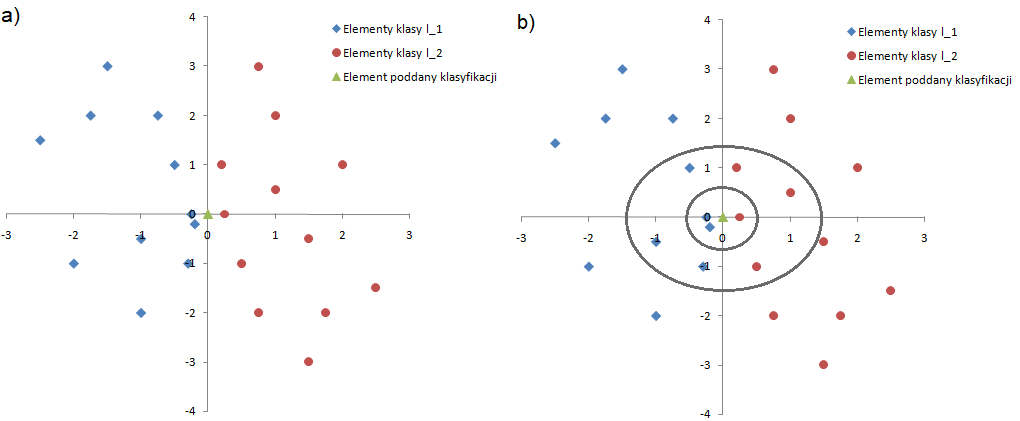
\includegraphics[scale=0.5]{kNN.PNG} 
\caption{Metoda $k$ - najbliższych sąsiadów. (źródło własne)}
\end{figure}
\end{center}

Na powyższym rysunku widzimy przykładowe zastosowanie algorytmu $k$-NN. Na pierwszym rysunku przedstawiony został zbiór treningowy z podziałem na dwie klasy (rąby, koła) oraz punkt, który będziemy chcieli przyporządkować do jednej z nich (trójkąt). Na drugim przedstawiono natomiast dwa koła, jedno prezentujące najbliższe sąsiedztwo dla $k = 3$, drugie dla $k = 9$. W obu przypadkach nowy punkt (trójkąt) zostanie przyporządkowany do klasy $l_1$. Warto jednak zauważyć, że znajduje się on na granicy dwóch klastrów przez co przy innym wyborze $k$ może zostać przyporządkowany do klasy $l_2$.

Opisana metoda przyporządkowuje wybranemu rekordowi najbardziej mu podobne. Wykorzystuje do tego miary odległości.

Najtrudniejszym zadaniem przy przeprowadzaniu algorytmu $k$-NN jest często wybór $k$. Jeżeli $k$ będzie zbyt małe - klasyfikator stanie się bardzo wrażliwy, jeżeli jednak $k$ będzie zbyt duże sąsiedztwo może zawierać zbyt dużo punktów z innych klas. Rozważając przypadek z rysunku 3.1 łatwo zauważyć, że nawet mała zmiana w obserwacjach zbioru treningowego może doprowadzić do zmiany wyniku.

\subsection{Algorytm k - średnich} 
Opis poniższego algorytmu oparty został na {\citep[Sec 2.3.1]{ascgdpds}}.

Algorytm k-średnich jest prostym i zarazem efektywnym algorytmem grupowania.

Głównym celem algorytmu jest podział pewnego zbioru $\mathit{X}$:
$$
\mathit{X} = \set{\mathbf{x}_i = (\mathbf{x}_{i1},\ldots,\mathbf{x}_{id}) : i \in \set{1,\ldots,N}},
$$
gdzie $\mathbf{x}_i$ jest $d$ - wymiarowym wektorem cech opisującym obiekt na podzbiory.

W wyniku grupowania $n$ - elementowego zbioru $\mathit{X}$ na $k$ podgrup jest macierz podziału $\mathbb{A}$ o wymiarach $k\times n$ . Każdy z elementów tej macierzy $a_{ik}$ oznacza stopień w jakim wektor $\mathbf{x}_k$ przynależy do grupy. Na wstępie algorytmu ustalamy wartość parametru $k$ jako liczbę grup, które zostaną wyodrębnione. Wybieramy $k$ reprezentantów, które stanowią prototypy grup.
\begin{center}
\begin{figure}[H]
\centering
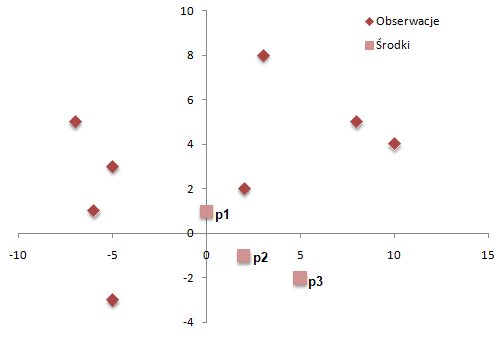
\includegraphics[scale=0.8]{ks_0.PNG} 
\caption{Metoda $k$-średnich. Wybór początkowych środków. (źródło własne)}
\end{figure}
\end{center}

W powyższym przykładzie (rysunek 3.2) wybranymi środkami są punkty $p1$, $p2$, $p3$. Kolejnym krokiem jest przypisanie każdego z elementów do najbliższej mu grupy.
\begin{center}
\begin{figure}[H]
\centering
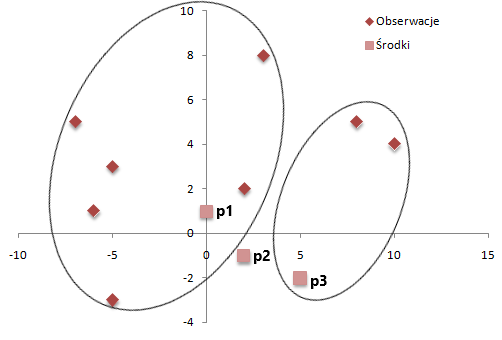
\includegraphics[scale=0.8]{ks_1.png} 
\caption{Metoda $k$-średnich. Przypisanie elementów do grup.(źródło własne)}
\end{figure}
\end{center}
Dla każdej z tak ustalonych grup obliczamy średnią arytmetyczną współrzędnych, które staną się kolejnymi środkami.
\begin{center}
\begin{figure}[H]
\centering
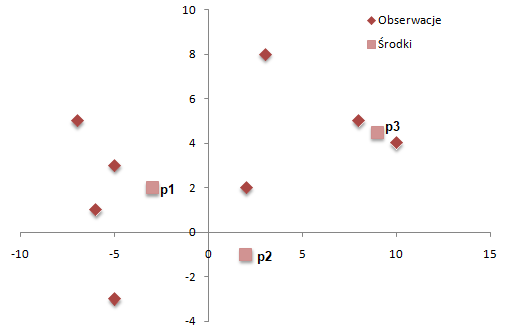
\includegraphics[scale=0.8]{ks_2.png} 
\caption{Metoda $k$-średnich. Wybór nowych środków.(źródło własne)}
\end{figure}
\end{center}
Kroki te są wykonywane do momentu występowania migracji między obiektami.
W algorytmie $k$-średnich liczba grup pozostaje więc niezmienną, zmienna jest tylko przynależność do grup.
W metodzie tej poszukiwanie optymalnego podziału odpowiada wyznaczaniu takich grup, które minimalizują następującą funkcje kryterialną:
$$
\J{\mathbf{p}}{\mathbb{A}} = \sum_{i=1}^k \sum_{k=1}^N a_{ki}\distance{\mathbf{p}_i}{\mathbf{x}_k}^2,
$$
gdzie 
\begin{itemize}
\item $\distance{\mathbf{p}_i}{\mathbf{x}_k}$ oznacza odległość elementu reprezentowanego przez wektor $\mathbf{x}$ od grupy wyznaczonej przez środek $\mathbf{p}$,
\item $N$ to liczebność zbioru $\mathit{X}$,
\item $\mathbb{A}$ oznacza macierz podziału.
\end{itemize}
 
\section{Szacowanie błędów obliczeń}
\subsection{Ocena dokładności metody}%RecommenderSystemsHandbook
Najczęściej używanymi miarami dokładności modelu są:
\begin{itemize}
\item błąd średni (Mean Error),
\item średni błąd bezwzględny (Mean Absolute Error),
\item średni błąd kwadratowy (Mean Squared Error).
\end{itemize}

Niech dla elementu $i$ ze zbioru $\mathit{P} = \set{x_1, \ldots, x_n}$ będzie dostarczona predykcja $\widehat{r}_i$. Aby ocenić jakość jej wyniku należy porównać ją ze znaną wartością $r_i$.

\begin{df}[Błąd średni {\citep[Sec 4.1.1]{rsh}}]
Średnim błędem nazywamy wartość wyrażenia:
$$
ME = \frac{1}{|\mathit{P}|}\sum_{x_i \in \mathit{P}}(\widehat{r}_i-r_i).
$$
\end{df}

\begin{df}[Średni błąd bezwzględny  {\citep[Sec 4.1.1]{rsh}}]
Średnim błędem bezwzględnym nazywamy wartość wyrażenia:
$$
MAD = \frac{1}{|\mathit{P}|}\sum_{x_i \in \mathit{P}}|\widehat{r}_i-r_i|.
$$
\end{df}

\begin{df}[Średni błąd kwadratowy  {\citep[Sec 4.1.1]{rsh}}]
Średnim błędem kwadratowym nazywamy wartość wyrażenia:
$$
MSE = \frac{1}{|\mathit{P}|}\sum_{x_i \in \mathit{P}}(\widehat{r}_i-r_i)^2.
$$
\end{df}
\begin{uwaga}{\citep[Sec 4.1.1]{rsh}}
Funkcja kwadratowa jest funkcją wypukłą co pozwala na dość częste zastępowanie średniego błędu kwadratowego przez średnią kwadratową błędów (Root Mean Squared Error (RMSE)):
$$
RMSE = \sqrt{MSE}
$$
Normalized RMSE (NRMSE) oraz Normalized MAE (NMAE) są znormalizownymi, przez użycie zakresu wartości $r_{max} - r_{min}$, wersjami błędów RMSE i MAE.
\end{uwaga}
Kolejnym rodzajem powszechnie używanego błędu, który pozwala na użycie sum ważonych jest średni błąd RMSE (Average RMSE).

\begin{df}[Średni błąd RMSE {\citep[Sec 4.1.1]{rsh}}]
Niech $w_i>0$ będzie wagę dla elementu $i$ oraz niech $\sum w_i = 1$.

Średnim błędem RMSE nazywamy wartość wyrażenia:
$$
ARMSE = \sqrt{\sum_{x_i\in \mathit{P}}w_{i}(\widehat{r}_i-r_i)^2}.
$$
\end{df}
\subsection{Ocena jakości modelu}
Ocenę jakości modelu przeprowadza się na zbiorze testowym. Dla każdego z rekordów jest znana jego etykieta. Rekordy te są poddawane działaniu modelu, a następnie etykiety przypisane rekordom przez model są porównywalne z rzeczywistymi wartościami etykiet.

W następnym kroku zliczana jest liczba rekordów poprawnie i niepoprawnie zaklasyfikowanych przez model, a wynik testu zostaje przestawiony w postaci macierzy pomyłek.
\begin{df}[Macierz pomyłek {\citep[Sec 4.8.1]{edmia}}]
Macierzą pomyłek nazywamy macierz kwadratową $ m \times m$ ($m$ oznacza liczbę etykiet), gdzie wiersze reprezentują etykiety faktyczne, natomiast kolumny etykiety przyporządkowane rekordom przez model. Element macierzy $\mathbb{F}$ oznacza liczbę rekordów z etykietą $E_i$, którym błędnie została przypisana etykieta $E_j$.
\begin{table}[H]
\begin{center}
\begin{tabular}{|r|r|r|} \hline
$\mathbb{F}$ & $E_1$ & $E_2$\\
\hline 
$E_1$ & $f_{11}$ & $f_{12}$ \\
\hline
$E_2$ & $f_{21}$ & $f_{22}$  \\
\hline
\end{tabular}
\end{center}
\caption{Macierz pomyłek.}
\label{tabelka}
\end{table}
\end{df}
\begin{uwaga}{\citep[Sec 4.8.1]{edmia}}
Często elementy macierzy pomyłek dla problemów klasyfikacji binarnej oznacza się symbolami : TP, TN, FN, FP. Oznaczenia te symbolizują cztery możliwe przypadki występujące w klasyfikacji binarnej. Załóżmy, że wyróżniamy klasę pozytywną (+) i negatywną (-). Wtedy :
\begin{itemize}
\item TP (ang. true - positive) - liczba pozytywnych rekordów testowych zaklasyfikowanych do klasy pozytywnej,
\item FN (ang. false - negative) - liczba pozytywnych rekordów testowych zaklasyfikowanych do klasy negatywnej,
\item FP (ang. false - positive) - liczba negatywnych rekordów testowych zaklasyfikowanych do klasy pozytywnej,
\item TN (ang. true - negative) - liczba negatywnych rekordów testowych zaklasyfikowanych do klasy negatywnej.
\end{itemize}
Macierz pomyłek przyjmuje wtedy postać:
\begin{table}[H]
\begin{center}
\begin{tabular}{|r|r|r|} \hline
$\mathbb{F}$ & $+$ & $-$\\
\hline
$+$ & $TP$ & $FN$ \\
\hline
$-$ & $FP$ & $TN$  \\
\hline
\end{tabular}
\end{center}
\caption{Macierz pomyłek - przypadek klasyfikacji binarnej.}
\label{tabelka}
\end{table}
\end{uwaga}
Poprzez analizę macierzy pomyłek bez problemu obliczymy łączną liczbę rekordów zaklasyfikowanych poprawnie oraz rekordów przypisanych błędnie przez klasyfikator. 

Analizę zawartości macierzy można rozszerzyć o dodatkową informację - koszt błędnej klasyfikacji (ang. misclassification cost).
\begin{df}[Koszt błędnej klasyfikacji {\citep[Sec 4.8.1]{edmia}}]
Oznaczmy przez $e_{ij}$ koszt błędnego zaklasyfikowania do klasy $E_j$ rekordu, który w rzeczywistości należy do klasy $E_i$.
Koszt poprawnej klasyfikacji oznaczmy przez $e_{ii}$ oraz załóżmy, że $\forall_{i}$ $ e_{ii} = 0$.
Dodatkowo niech $f_{t}$ oznacza liczbę wszystkich przykładów testowych, $f_{p}$ liczbę poprawnie zaklasyfikowanych rekordów testowych oraz $f_{p} = \sum_{i=1}^m f_{ii}$, $f_{b}$ niech natomiast oznacza liczbę błędnych klasyfikacji i $f_{b} = f_{t} - f_{p}$.

Kosztem błędnej klasyfikacji $E(f_{b})$ nazywamy sumę:
$$
E(f_{b}) = \sum_{i=1}^m \sum_{j=1}^m f_{ij} \cdot e_{ij}.
$$
\end{df}

W przypadkach, gdy błędne zaklasyfikowania rekordów nie różnią się kosztami, do oceny jakości klasyfikatora można wykorzystać miary takie jak trafność klasyfikacji (ang. accuracy) oraz błąd klasyfikacji (ang. error rat).
\begin{df}[Trafność klasyfikacji {\citep[Sec 4.8.1]{edmia}}]
Trafnością klasyfikacji nazywamy stosunek liczby popranie zaklasyfikowanych rekordów testowych do łącznej liczby rekordów testowych:
$$
TR= \frac{f_p}{f_t} = \frac{\sum_{i=1}^m f_{ii}}{f_t}.
$$
\end{df}
\begin{df}[Błąd klasyfikacji {\citep[Sec 4.8.1]{edmia}}]
Błędem klasyfikacji nazywamy stosunek liczby błędnie zaklasyfikowanych rekordów testowych do łącznej liczby rekordów testowych:
$$
BK = \frac{f_b}{f_t}=\frac{\sum_{i=1}^m \sum_{j=1}^m f_{ij}}{f_t}=1 - \frac{f_p}{f_t}.
$$
\end{df}
\begin{uwaga}{\citep[Sec 4.8.1]{edmia}}
Innymi miarami, które można wywnioskować bezpośrednio z macierzy pomyłek dla klasyfikacji binarnej (tabla 3.2) są:
\begin{itemize}
\item współczynnik $TP$ (czułość):
$$
WTP = \frac{TP}{TP + FN},
$$
\item współczynnik $FP$:
$$
WFP = \frac{FP}{FP + TN},
$$
\item współczynnik $TN$ (specyficzność):
$$
WTN = \frac{TN}{FP + TN},
$$
\item precyzja:
$$
precyzja = \frac{TP}{TP + FP},
$$
\item zwrot:
$$
zwrot = \frac{TP}{TP + FN},
$$
\item $F$-miara:
$$
F - miara = \frac{2 \cdot precyzja \cdot zwrot}{precyzja \cdot zwrot}.
$$
\end{itemize}
\end{uwaga}

\chapter{Modele tworzenia rekomendacji}

W niniejszym rozdziale zajmiemy się formalnym zdefiniowanie zadania, które ukrywa się pod nazwą tworzenia rekomendacji. Do jego poprawnego określenia będą przydatne następujące pojęcia.

\begin{df}[Przedmiot {\citep[Sec 1.3]{kidzinski}}]
 Przedmiotem nazwiemy klasę obiektów tego samego typu, nierozróżnialnych dla obserwatora i reprezentowanych przez co najmniej jeden element. W dalszej części pracy zbiór przedmiotów będziemy oznaczać przez $\setPrzedmioty$.
\end{df}

Przedmioty stanowią podstawową grupę elementów w rozważaniach systemach rekomendujących. 

\begin{df}[Użytkownik {\citep[Sec 1.3]{kidzinski}}]
Użytkownikiem nazywamy osobę zdolną do przedstawienia własnej oceny wybranego przedmiotu. W dalszej części pracy zbiór użytkowników będziemy oznaczać przez $\setUzytkownicy$.
\end{df}

W pracy \citep{kidzinski} użyty jest zawsze ten sam zbiór ocen, jednak łatwo możemy pokusić się o jego uogólnioną definicję.

\begin{df}[Zbiór ocen {\citep[Sec 1.3]{kidzinski}}]
Podzbiór skończony zbioru $\setN$ lub $\setN \cup \set{0}$ nazywamy zbiorem ocen dla przedmiotów. W dalszej części pracy zbiór ocen będziemy oznaczać przez $\setOceny$.
\end{df} 

\begin{df}[Macierz preferencji {\citep[Sec 1.3]{kidzinski}}]
Rozważmy zbiór przedmiotów o liczności $n$ oraz grupę użytkowników o liczności $m$. Macierzą preferencji $M$ nazwiemy macierz o wymiarach $n \times m$ i wartościach w ustalonym zbiorze ocen.
\end{df}

Z uwagi na to, że przedmioty jako wytwory świata rzeczywistego są niemożliwe do opisania za pomocą skończonej liczby cech  rozważa się ich skończoną reprezentację nazywaną wektorem własności.

\begin{df}[Własność {\citep[Sec 1.3]{kidzinski}}]
Własnością nazwiemy cechę wyrażoną za pomocą wartości liczbowej lub pewnej zmiennej kategorycznej, która reprezentuje cechę przedmiotu istotną dla użytkownika w procesie tworzenia oceny. Zbiór wszystkich własności w rozważanym modelu oznaczamy $\setWlasnosci$. Dla każdej $w \in \setWlasnosci$ poprzez $V_w$ rozumiemy zbiór wszystkich dopuszczalnych wartości własności $w$.
\end{df}

\begin{df}[Funkcja anotująca {\citep[Sec 1.3]{kidzinski}}]
Funkcją anotującą własność $w \in \setWlasnosci$ nazwiemy funkcję 
$$
a_w \colon \setPrzedmioty \to V_w.
$$
\end{df}

Mając na uwadze, że zbiór $\setWlasnosci$ jest skończony (jak również zbiór $\setPrzedmioty$) można utożsamiać funkcję anotującą z wektorem o długości $|\setWlasnosci|$ nazywanym wektorem własności.

\begin{df}[Funkcja przynależności {\citep[Sec 4.2]{msi}}]
Funkcja przynależności nazywamy funkcję
$$
\mu_{\setWlasnosci}(p_i): \setPrzedmioty \to [0,1]
$$
określa stopień przynależności przedmiotu $p_i \in \setPrzedmioty$ do zbioru $\setWlasnosci=\set{w_k}$.
\end{df}

\begin{df}[Problem tworzenia rekomendacji {\citep[Sec 1.3]{kidzinski}}]
Rozważmy pewien zbiór przedmiotów $\setPrzedmioty$, pewien zbiór użytkowników $\setUzytkownicy$ oraz pewien zbiór ocen $\setOceny$. Niech ponadto $R$ będzie funkcją taką, że:
$$ 
R: \setPrzedmioty \times \setUzytkownicy \to \setOceny .
$$
Załóżmy, że dla funkcji $R$ znane są wartości dla pewnych par przedmiotów i użytkowników. Naszym zadaniem jest zaproponowanie sposobu predykcji brakujących wartości funkcji $R$ w sposób minimalizujący wybrany funkcjonał błędu. 
\end{df}

Przyjrzyjmy się następującemu przykładowi, który ilustruje istotę problemu.

\begin{przyklad}
Niech zbiór przedmiotów będzie w tym przypadku zbiorem sześciu książek. Zatem $\setPrzedmioty = \set{p_1, p_2, p_3, p_4, p_5, p_6}$, gdzie $p_i$ dla $i \in \set{1,2,3,4,5,6}$ oznacza $i$ - tą książkę. Zbiór użytkowników niech będzie zbiorem czytelników. Zatem 
\\$\setUzytkownicy = \{u_1, u_2, u_3, u_4, u_5, u_6\}$, gdzie $u_i$ dla $i \in \set{1,2,3,4,5,6}$ oznacza $i$ - tego czytelnika.
Poniższa tabela to macierz preferencji dla ustalonego zbioru $\setPrzedmioty$ i ustalonego zbioru $\setUzytkownicy$. Znak '?' oznacza brakujące wartości funkcji $R$, zatem czytelnik danej książki nie czytał lub czytał lecz jego ocena jest nieznana.
\begin{center}
\begin{tabular}{|r|r|r|r|r|r|r|r|} \hline
\textbf{Czytelnicy} & & $\mathbf{u_1}$ & $\mathbf{u_2}$ & $\mathbf{u_3}$ & $\mathbf{u_4}$ & $\mathbf{u_5}$ & $\mathbf{u_6}$ \\
\hline
\hline
\textbf{Książki} &$\mathbf{p_1}$ & 6 & 3 & \textbf{?} & 6 & 4 & \textbf{?} \\
\hline
&$\mathbf{p_2}$ & \textbf{?} & 6 & 6 & 5 & 6 & \textbf{?} \\
\hline
&$\mathbf{p_3}$ & 7 & 7 & 8 & 7 & 8 & 9  \\
\hline
&$\mathbf{p_4}$ & 8 & 10 & 10 & 7 & 6 & 8 \\
\hline
&$\mathbf{p_5}$ & 9 & 6 & 6 & 6 & 6 & \textbf{?} \\
\hline
&$\mathbf{p_6}$ & 5 & 7 & 7 & 5 & 4 & 2 \\
\hline
\end{tabular}.
\end{center}

Zadaniem jest przewidzieć brakujące wartości funkcji $R$, czyli oceny nadane przez użytkowników w sposób minimalizujący błąd popełniany przez model.
\end{przyklad}
\begin{uwaga}[Podział systemów rekomendujących]
Podziału systemów rekomendujących dokonujemy ze względu na zakres wykorzystywanych informacji. Wyróżniamy:
\begin{itemize}
\item systemy rekomendujące oparte na treści,
\item filtrowanie kolaboratywne,
\item systemy rekomendujące kontekstowe.
\end{itemize}

W przypadku systemów rekomendujących opartych na treści predykcja jest dokonywana na podstawie ocen wystawionych przedmiotom przez użytkowników oraz wektorów własności rozważanych przedmiotów. 

W filtrowaniu kolaboratywnym wektory cech zostają pominięte, a predykcja dokonywana jest na podstawie ocen. Wyróżniamy dwa typy filtrowania kolaboratywnego:
\begin{itemize}
\item filtrowanie oparte na użytkownikach

Niech $\mathbf{u}_1 = [o_{1,1}, \ldots, o_{1,n}]$ oraz $\mathbf{u}_2 = [o_{2,1}, \ldots, o_{2,n}]$ będą wektorami opisującymi odpowiednio użytkownika $u_1$ i $u_2$. Elementami wektorów są wartości funkcji R w przypadkach, gdzie zarówno użytkownik $u_1$, jak i $u_2$ ocenili ten sam przedmiot. Główne założenie filtrowania kolaboratywnego opartego na użytkownikach mówi, że jeżeli odległość między wektorami $\mathbf{u}_1$ i $\mathbf{u}_2$ jest mała oraz użytkownik $u_1$ ocenił pewien przedmiot dla którego użytkownik $u_2$ jeszcze nie wystawił oceny, to prawdopodobnie ocena użytkownika $u_2$ będzie podobna do oceny użytkownika $u_1$.
\item filtrowanie oparte na elementach

Niech $\mathbf{p}_1 = [o_{1,1}, \ldots, o_{1,n}]$ oraz $\mathbf{p}_2 = [o_{2,1}, \ldots, o_{2,n}]$ będą wektorami opisującymi odpowiednio przedmiot $p_1$ i $p_2$. Elementami wektorów są wartości funkcji R w przypadkach, gdzie przedmiot $p_1$, jak i $p_2$ został oceniony przez tego samego użytkownika. Główne założenie filtrowania kolaboratywnego opartego na elementach mówi, że jeżeli odległość między wektorami $\mathbf{p}_1$ i $\mathbf{p}_2$ jest mała oraz użytkownik ocenił w pewien sposób przedmiot $p_1$ w przeszłości to będzie skłonny w podobny sposób ocenić przedmiot $p_2$.
\end{itemize}

Systemy rekomendujące kontekstowe są natomiast systemami rekomendującymi opartymi na treści w których zostaje uwzględniony dodatkowy wymiar - kontekst.
\end{uwaga}

\section{Systemy rekomendujące oparte na treści - Content-based recommender systems}
Rozważania zawarte w tej sekcji zostały przeprowadzone na podstawie książki Gorakala S. K.: \textit{Building Recommendation Engines} {\citep[Sec 3]{bre}} oraz kursu autorstwa Andrew N.: \textit{Recommender Systems} {\citep{rs}}.
\bigskip

Systemy oparte na treści wyróżnia ukierunkowanie na spersonalizowany poziom użytkownika oraz treść produktu. Metoda ta opiera się na obliczaniu podobieństw oraz wykorzystuje techniki uczenia maszynowego, takie jak klasyfikacja.

\begin{algorytm}
W metodzie celem stworzenia rekomendacji i wygenerowania listy przedmiotów, które mogę być odpowiednie użytkownikowi opieramy się na treści rozważanych elementów. Algorytm tego rodzaju rekomendacji możemy przedstawić w następujących krokach:
\begin{enumerate}
\item stworzenie wektora własności $\mathbf{w} = [w_1, \ldots, w_n]$, $n \in \setN$, gdzie $\forall_{i \in \set{1, \ldots, n}} \: w_i \in \setWlasnosci$,

\item wygenerowanie profilów produktów - stworzenie wektorów własności $\mathbf{w}_{p_i}$ gdzie poszczególne elementy wektora określają przynależność przedmiotu $p_i$, $i \in \setN$ do odpowiednich elementów wektora własności $\mathbf{w}$ określonego w kroku 1.,

\item wygenerowanie profilów użytkowników - stworzenie wektorów własności $\mathbf{w}_{u_j}$ przypisanych użytkownikom, gdzie poszczególne elementy wektora określają przynależność opinii użytkownika $u_j$, $j \in \setN$ do elementów wektora własności $\mathbf{w}$ określonego w kroku 1.,

\item obliczmy ocenę $\widehat{o}_{j,i}$ jaką użytkownik $j$ wystawiłby dla przedmiotu $i$, którego wcześniej nie oceniał za pomocą funkcji
$$
\widehat{o}_{j,i} = \mathbf{w}_{u_j}^T \mathbf{w}_{p_i},
$$

\item porównując otrzymane w kroku 3. oceny dokonujemy rekomendacji nowego przedmiotu.
\end{enumerate}
\end{algorytm}

\begin{przyklad}
Niech wektor własności będzie określony następująco $\mathbf{w} = [w_1, w_2]$, a każdy z elementów wektora $\mathbf{w}$ niech reprezentuje inny gatunek. Poniższa tabela określa przynależność (w przedziale $[0,1]$) każdej z książek do elementów wektora własności $w$. 
\begin{center}
\begin{tabular}{|r|r|r|r|} \hline
\textbf{Gatunki} & & $\mathbf{w_1}$ & $\mathbf{w_2}$  \\
\hline
\hline
\textbf{Książki} &$\mathbf{p_1}$ & 0.9 & 0 \\
\hline
&$\mathbf{p_2}$ & 1 & 0.01  \\
\hline
&$\mathbf{p_3}$ & 0.99 & 0 \\
\hline
&$\mathbf{p_4}$ & 0.1 & 1 \\
\hline
&$\mathbf{p_5}$ & 0 & 0.9 \\
\hline
&$\mathbf{p_6}$ & 0.8 & 0.3 \\
\hline
\end{tabular}
\end{center}
Dodatkowo zakładamy, że istnieje gatunek $w_0$, którego cechy reprezentują wszystkie książki oraz dla każdej z książek $w_0=1$.

Zatem wektor własności odpowiadające poszczególnym książkom mają postać
$$
\mathbf{w}_{p_1} = [1, 0.9, 0] ^ T, \: \mathbf{w}_{p_2} = [1, 1, 0.01] ^ T, \: \mathbf{w}_{p_3} = [1, 0.99, 0] ^ T,
$$
$$
\mathbf{w}_{p_4} = [1, 0.1, 1] ^ T, \: \mathbf{w}_{p_5} = [1, 0, 0.9] ^ T, \: \mathbf{w}_{p_6} = [1, 0.8, 0.3] ^ T.
$$
Dla każdego użytkownika $j$ wyznaczamy wektor parametrów $\mathbf{w}_{u_j} \in \setR^3$, który przedstawia przynależność (w przedziale $[0,1]$) opinii użytkownika do elementów wektora własności. 

Preferencje czytelników zostaną więc opisane za pomocą wektorów:
$$
\mathbf{w}_{u_1}, \: \mathbf{w}_{u_2}, \: \mathbf{w}_{u_3}, \: \mathbf{w}_{u_4}, \: \mathbf{w}_{u_5}, \: \mathbf{w}_{u_6}.
$$
Obliczmy ocenę jaką książce $p_3$ wystawiłby użytkownik $u_1$ przy założeniu, że wektor preferencji użytkownika $u_1$ jest postaci $\mathbf{w}_{u_1}= [0,5,0]^T$. Użytkownik ten preferuje więc książki gatunku $w_1$, gdy książki gatunków $w_0$ i $w_2$ są dla niego nieatrakcyjne.
Zatem:
$$
\widehat{o}_{1,3} = \mathbf{w}_{u_1}^T \mathbf{w}_{p_3} = [0,5,0] \cdot [1, 0.99, 0] ^ T = 0 \cdot 1 + 5 \cdot 0,99 + 0 \cdot 0 = 4,95.
$$

Przewidywaną oceną jest zatem $4,95$. 

Po przeprowadzeniu podobnych obliczeń dla wszystkich wcześniej nieznanych ocen możemy zarekomendować naszemu użytkownikowi nową lekturę.
\end{przyklad}

\subsection{Wygenerowanie profilu dokumentu tekstowego - algorytm TFIDF}
Rozważania na temat algorytmu TFIDF zawarte w tym rozdziale zostały przeprowadzone na podstawie książki \textit{Recommender Systems Handbook} {\citep[Sec 3.3.1.1]{rsh}}.
\bigskip
\bigskip

W większość systemów rekomendacji opartych na treści używamy gotowych modeli wyszukujących. 

W przypadku rozważań przeprowadzanych na dokumentach tekstowych jednym z najbardziej popularnych jest model przestrzeni wektorowej (\textit{ang. Vector Space Model}) z algorytmem TFIDF. 
\bigskip

Niech $\setPrzedmioty = \set{p_1, p_2, \ldots ,p_n}, n\in \setN$ będzie zestawem analizowanych przedmiotów. $W = \set{w_1, w_2, \ldots ,w_n}, \: n\in \setN $ niech będzie zbiorem rozważanych własności.

\begin{df}[Model przestrzeni wektorowej {\citep[Sec 3.3.1.1]{rsh}}]
Modelem przestrzeni wektorowej nazywamy formę reprezentacji przedmiotów, w której przedmiot $p_i$ jest reprezentowany przez wektor z przestrzeni $n$-wymiarowej, a każdy z $n$ wymiarów reprezentuje jedną z rozważanych własności przedmiotu. 
\end{df}

Dla danych w formie dokumentów tekstowych przedmiotem $p_i$ jest dokument (artykuł, książka), natomiast własnościami, które charakteryzują temat dokumentu są słowa. Mając na uwadze te założenia możemy zdefiniować kolejne elementy algorytmu $TFIDF$.

\begin{df}[Liczność {\citep[Sec 3.3.1.1]{rsh}}]
Licznością $f_{k,j}$ nazywamy liczbę wystąpień własności $w_k$ w przedmiocie $p_j$.
\end{df}

\begin{df}[TF {\citep[Sec 3.3.1.1]{rsh}}]
$TF$ (ang. \textit{term frequency}) nazywamy funkcję przedstawiającą zależność własności $w_k$ od przedmiotu $p_j$:
$$
TF(w_k, p_j)=\frac{f_{k,j}}{\max_{z}f_{z,j}},
$$
gdzie:
\begin{itemize}
\item $\max_{z}f_{z,i}$ - maksymalna w odniesieniu do wszystkich wartości $w_z \in \setWlasnosci$, $z \in \set{1, \ldots, n}$, które pojawiły się w przedmiocie $p_i$, liczność wystąpień własności. 
\end{itemize}
\end{df}

\begin{df}[IDF {\citep[Sec 3.3.1.1]{rsh}}]
$IDF$ (ang. \textit{inverse dokument frequency}) nazywamy funkcję:
$$
IDF(w_k) = \log \frac{N}{n_k},
$$
gdzie:
\begin{itemize}
\item $N$ - całkowita liczba przedmiotów w zbiorze $\setPrzedmioty$,
\item $n_k$ - liczba przedmiotów w których własność $w_k$, $k \in \set{1, \ldots, n}$ wystąpiła przynajmniej raz.
\end{itemize}
\end{df}

\begin{df}[TFIDF {\citep[Sec 3.3.1.1]{rsh}}]
$TFIDF$ (ang. \textit{TF – term frequency, IDF - inverse document frequency}) nazywamy funkcję:
$$
TFIDF(w_k, p_i) = TF(w_k, p_i) \cdot IDF(w_k).
$$
\end{df}

\begin{df}[Waga własności w przedmiocie]
Wagą własności $w_k$ w przedmiocie $p_i$ nazywamy wartość:
$$
s_{k,i} = \frac{TFIDF(w_k, p_i)}{\sqrt{ \sum_{j=1}^{|W|}{TFIDF(w_j, p_i)}^2}}.
$$
\end{df}

\begin{uwaga}
Każdy z dokumentów $p_i, \: i\in\set{1,\ldots,n} $ przedstawiamy jako wektor wag własności (słowa) $w_k$ w przedmiocie $p_i$. Zatem $ p_i = [s_{1i}, s_{2i},...,s_{ni}] $.
\end{uwaga}

\section{Filtrowanie kolaboratywne - Collaborative filtering}
Rozważania na temat filtrowania kolaboratywnego zostały przeprowadzone na podstawie książki Gorakala S. K.: \textit{Building Recommendation Engines} {\citep[Sec 3]{bre}}.
\bigskip

Podejście kolaboratywne omija niektóre ograniczenia występujące w metodach opartych na treści. Dzięki temu systemowi możemy dokonywać rekomendacji z pominięciem wektorów preferencji. 

\subsection{Filtrowanie kolaboratywne oparte na użytkowniku}

\begin{algorytm}
Stworzenie rekomendacji filtrowania kolaboratywnego opartej na użytkownikach wykonamy w następujących krokach:
\begin{enumerate}
\item wybór użytkowników $u_j, u_k \in \setUzytkownicy$, $j,k \in \setN$, między którymi chcemy obliczyć podobieństwo,
\item wybór przedmiotów $p_i \in \setPrzedmioty$, $i \in \setN$, dla których znane wartości funkcji $R(p_i,u_j)$ i $R(p_i,u_k)$,
\item stworzenie wektorów ocen $o_{j,k}^{(j)}$ i $o_{j,k}^{(k)}$ dla użytkowników $u_j$ i $u_k$ wybranych w kroku 1., których elementy stanowią wartości $R(p_i,u_j)$ oraz $R(p_i,u_k)$, gdzie $p_i$ to przedmioty wybrane w kroku 2.,
\item wyznaczenie odległości między czytelnikami $u_j$ i $u_k$ - najczęstszymi stosowanymi podejściami do obliczania odległości są metryka euklidesowa i współczynnik korelacji Pearsona,
\item wyznaczenie macierzy odległości $\mathbb{U}_1$ między wszystkimi czytelnikami ze zbioru $\setUzytkownicy$,
\item wyznaczenie macierzy odległości $\mathbb{U}_2$ między czytelnikami poprzez normalizację danych w celu uzyskania wartości z przedziału $[0,1]$, wyrazy macierzy przyjmują wartości:
$$
u_{ij}^{(2)} = \frac{u_{ij}^{(1)}}{max_{o_i} \set{o_i : o_i \in \setOceny,\: i \in \setN } - min_{o_i} \set{o_i : o_i \in \setOceny, \: i \in \setN}},
$$
gdzie $u_{ij}^{(1)}$ i $u_{ij}^{(2)}$ są odpowiednio elementami macierzy $\mathbb{U}_1$ i $\mathbb{U}_2$, $i,j \in \setN$,
\item wyznaczenie macierzy podobieństwa $\mathbb{U}_3$ między użytkownikami - zakładając, że największa wartość prawdopodobieństwa to $1$ macierz podobieństwa przyjmuje wartości:
$$
u_{ij}^{(3)} = 1 - u_{ij}^{(2)},
$$
gdzie $u_{ij}^{(2)}$ i $u_{ij}^{(3)}$ są odpowiednio elementami macierzy $\mathbb{U}_2$ i $\mathbb{U}_3$,
\item wyestymowanie nieznanych wartości funkcji $R$ dla $u_j \in \setUzytkownicy$, $j \in \setN$ oraz $p_i \in \setPrzedmioty$, $i \in \setN$  - niech $u_j$ będzie konkretnie ustalonym użytkownikiem, w celu obliczenia brakujących wartości funkcji $R$ dla użytkownika $u_j$ obliczmy średnią ważoną wykorzystując oceny i przyjmując wartości podobieństwa między $u_j$ i innymi użytkownikami jako wagi.
\end{enumerate}
\end{algorytm}

W celu dokładniejszego zrozumienia rozważmy ponownie przykład 4.1.

\begin{przyklad}
Chcąc obliczyć podobieństwo między użytkownikiem $u_2$ i $u_3$ wybierzmy książki, które zostały przeczytane przez obu użytkowników. W tym przypadku są to: $p_2$, $p_3$, $p_4$, $p_5$, $p_6$. Wektorami ocen uwzględniającymi książki ocenione przez obu użytkowników są więc odpowiednio dla użytkownika $u_2$ wektor $o_{2,3} ^{(2)} = [6, 7, 10, 6, 7] ^ T$ oraz dla użytkownika $u_3$ wektor $o_{2,3}^{(3)} = [6, 8, 10, 6, 7] ^ T$.

Posługując się odległością euklidesową obliczamy odległość między użytkownikami $u_2$ i $u_3$: 
$$
d_{e}(o_{2,3}^{(2)},o_{2,3}^{(3)}) = \sqrt{(6-6)^2 + (7-8)^2 + (10-10)^2 + (6-6)^2 + (7-7)^2} = \sqrt{1} = 1.
$$

Postępując w podobny sposób dla każdej z par użytkowników otrzymamy następującą macierz odległości $\mathbb{U}_1$:
\begin{center}
\begin{tabular}{|r|r|r|r|r|r|r|} \hline
$\mathbb{U}_1$ & $\mathbf{u_1}$ & $\mathbf{u_2}$ & $\mathbf{u_3}$ & $\mathbf{u_4}$ & $\mathbf{u_5}$ & $\mathbf{u_6}$ \\
\hline
$\mathbf{u_1}$ & 0 & 5,099 & 4,243 & 3 & 4,359 & 3,606 \\
\hline
$\mathbf{u_2}$ & 5,099 & 0 & 1 & 4,796 & 5,196 & 5,745 \\
\hline
$\mathbf{u_3}$ & 4,243 & 1 & 0 & 3,873 & 5 & 5,477 \\
\hline
$\mathbf{u_4}$ & 3 & 4,796 & 3,873 & 0 & 2,828 & 3,742  \\
\hline 
$\mathbf{u_5}$ & 4,359 & 5,196 & 5 & 2,828 & 0 & 3 \\
\hline 
$\mathbf{u_6}$ & 3,606 & 5,745 & 5,477 & 3,742 & 3 & 0  \\
\hline 
\end{tabular}.
\end{center}
W procesie normalizacji danych dzielimy elementy macierzy przez 
$$
(max\{0,1,2,3,4,5,6,7,8,9,10\} - min\{0,1,2,3,4,5,6,7,8,9,10\}) = 10
$$ 
i otrzymujemy macierz $\mathbb{U}_2$ postaci:
\begin{center}
\begin{tabular}{|r|r|r|r|r|r|r|} \hline
$\mathbb{U}_2$ & $\mathbf{u_1}$ & $\mathbf{u_2}$ & $\mathbf{u_3}$ & $\mathbf{u_4}$ & $\mathbf{u_5}$ & $\mathbf{u_6}$ \\
\hline
$\mathbf{u_1}$ & 0 & 0,5099 & 0,4243 & 0,3 & 0,4359 & 0,3606 \\
\hline
$\mathbf{u_2}$ & 0,5099 & 0 & 0,1 & 0,4796 & 0,5196 & 0,5745 \\
\hline
$\mathbf{u_3}$ & 0,4243 & 0,1 & 0 & 0,3873 & 0,5 & 0,5477 \\
\hline
$\mathbf{u_4}$ & 0,3 & 0,4796 & 0,3873 & 0 & 0,2828 & 0,3742 \\ 
\hline 
$\mathbf{u_5}$ & 0,4359 & 0,5196 & 0,5 & 0,2828 & 0 & 0,3 \\
\hline 
$\mathbf{u_6}$ & 0,3606 & 0,5745 & 0,5477 & 0,3742 & 0,3 & 0 \\ 
\hline 
\end{tabular}.
\end{center}
Macierz podobieństwa $\mathbb{U}_3$ przyjmuje więc wartości:
\begin{center}
\begin{tabular}{|r|r|r|r|r|r|r|} \hline
$\mathbb{U}_3$ & $\mathbf{u_1}$ & $\mathbf{u_2}$ & $\mathbf{u_3}$ & $\mathbf{u_4}$ & $\mathbf{u_5}$ & $\mathbf{u_6}$ \\
\hline
$\mathbf{u_1}$ & 1 & 0,4901 & 0,5757 & 0,7 & 0,5641 & 0,6394 \\
\hline
$\mathbf{u_2}$ & 0,4901 & 1 & 0,9 & 0,5204 & 0,4804 & 0,4255 \\
\hline
$\mathbf{u_3}$ & 0,5757 & 0,9 & 1 & 0.6127 & 0,5 & 0,4523 \\
\hline
$\mathbf{u_4}$ & 0,7 & 0,5204 & 0.6127 & 1 & 0,7172 & 0,6258 \\ 
\hline 
$\mathbf{u_5}$ & 0,5641 & 0,4804 & 0,5 & 0,7172 & 1 & 0,7 \\
\hline 
$\mathbf{u_6}$ & 0,6394 & 0,4255 & 0,4523 & 0,6258 & 0,7 & 1 \\ 
\hline 
\end{tabular}.
\end{center}
Obliczamy ocenę jaką użytkownik $u_1$ zaproponuje dla książki $p_2$:
$$
\frac{0,4901 \cdot 6 + 0,5757 \cdot 6 + 0,7 \cdot 5 + 0,5641 \cdot 6}{0,4901 + 0,5757  + 0,7  + 0,5641} = 5,7
$$

Na podstawie metody filtrowania kolaboratywnego opartej na użytkownikach wnioskujemy, że użytkownik $u_1$ wystawiłby książce $p_2$ ocenę $5,7$.

Postępując w analogiczny sposób przewidzimy wszystkie brakujące oceny :
\begin{center}
\begin{tabular}{|r|r|r|r|r|r|r|r|} \hline
\textbf{Czytelnicy} & & $\mathbf{u_1}$ & $\mathbf{u_2}$ & $\mathbf{u_3}$ & $\mathbf{u_4}$ & $\mathbf{u_5}$ & $\mathbf{u_6}$ \\
\hline
\hline
\textbf{Książki} &$\mathbf{s_1}$ & 6 & 3 & \textbf{4,57} & 6 & 4 & \textbf{4,88} \\
\hline
&$\mathbf{s_2}$ & \textbf{5,7} & 6 & 6 & 5 & 6 & \textbf{5,72} \\
\hline
&$\mathbf{s_3}$ & 7 & 7 & 8 & 7 & 8 & 9 \\
\hline
&$\mathbf{s_4}$ & 8 & 10 & 10 & 7 & 6 & 8 \\
\hline
&$\mathbf{s_5}$ & 9 & 6 & 6 & 6 & 6 & \textbf{6,67}  \\
\hline
&$\mathbf{s_6}$ & 5 & 7 & 7 & 5 & 4 & 2 \\
\hline
\end{tabular}.
\end{center}
Możemy więc wnioskować, że w tym przypadku dla użytkownika $u_3$ książka $p_1$ prawdopodobnie nie będzie zbyt atrakcyjna. Użytkownik $u_6$, natomiast, z chęcią przeczyta książkę $p_5$. 
\end{przyklad}

\subsection{Filtrowanie kolaboratywne oparte na  elementach}
W przypadku filtrowania kolaboratywnego opartego na elementach wartości podobieństwa między użytkownikami zostaje zastąpiona przez wartości podobieństwa między elementami.

\begin{algorytm}
W tym rodzaju rekomendacji należy wykonać następujące kroki:
\begin{enumerate}
\item wybór przedmiotów $p_i, p_k \in \setPrzedmioty$, $i,k \in \setN$, dla których znamy wartość funkcji $R(p_i,u_j)$ oraz wartość funkcji $R(p_k,u_j)$, gdzie $u_j$ jest użytkownikiem, który wystawia ocenę w obu przypadkach,
\item stworzenie wektorów ocen $\overline{o^{(p_i)}}$ i $\overline{o^{(p_k)}}$ dla przedmiotów $p_i$ i $p_k$ wybranych w kroku 2., których elementy stanowią stanowią wartości funkcji $R$ dla użytkownika $u_j$,
\item wyznaczenie odległości między przedmiotami $p_i$ i $p_k$ - najczęstszymi stosowanymi podejściami do obliczania odległości jest podobieństwo kosinusów,
\item wyznaczenie macierzy podobieństwa $\mathbb{P}$ między wszystkimi przedmiotami $\setPrzedmioty$,
\item wyestymowanie nieznanych wartości funkcji $R$ dla $u_j \in \setUzytkownicy$, $j \in \setN$ oraz $p_i \in \setPrzedmioty$, $i \in \setN$  - niech $p_i$ będzie konkretnie ustalonym przedmiotem oraz $u_j$ będzie konkretnie ustalonym użytkownikiem, w celu obliczenia brakujących wartości funkcji $R$ dla $u_j$ i $p_i$ obliczmy średnią ważoną wykorzystując oceny oraz przyjmując wartości podobieństwa między $p_i$ i innymi przedmiotami ocenionymi przez użytkownika jako wagi.
\end{enumerate}
\end{algorytm}

\begin{przyklad}
Aby obliczyć podobieństwo między książkami $p_1$ i $p_2$ wyznaczmy wektory ocen w których uwzględnimy przypadki, gdzie jeden użytkownik ocenił obie pozycje.

Zatem: $\overline{o^{(p_1)}} = [3, 6, 4]^T$, $\overline{o^{(p_2)}} =[6, 5, 6]^T$.

Następnie używając wzoru na podobieństwo kosinusowe obliczamy podobieństwo między wybranymi książkami
$$
sim(p_1,p_2) = \frac{\overline{o^{(p_1)}} \cdot \overline{o^{(p_2)}}}{|o^{(p_1)}||o^{(p_2)}|} = \frac{3 \cdot 6 + 6 \cdot 5 + 4 \cdot 6}{\sqrt{6^2 + 3^2 + 6^2 + 4^2} \sqrt{6^2 + 6^2 + 5^2 + 6^2}} = 0,6339.
$$
Postępując w analogiczny sposób otrzymamy macierz podobieństwa:
\begin{center}
\begin{tabular}{|r|r|r|r|r|r|r|r|} \hline
$\mathbb{P}$ & $\mathbf{p_1}$ & $\mathbf{p_2}$ & $\mathbf{p_3}$ & $\mathbf{p_4}$ & $\mathbf{p_5}$ & $\mathbf{p_6}$ \\
\hline
$\mathbf{p_1}$ & 1 & 0,6339 & 0,7372 & 0,7195 & 0,8935 & 0,7599 \\
\hline
$\mathbf{p_2}$ & 0,6339 & 1 & 0,7951 & 0,8150 & 0,7977 & 0,8898 \\
\hline
$\mathbf{p_3}$ & 0,7372 & 0,7951 & 1 & 0,9780 & 0,8586 & 0,9200 \\
\hline
$\mathbf{p_4}$ & 0,7195 & 0,8150 & 0,9780 & 1 & 0,8860 & 0,9681 \\
\hline 
$\mathbf{p_5}$ & 0,8935 & 0,7977 & 0,8586 & 0,8860 & 1 & 0,9413 \\
\hline 
$\mathbf{p_6}$ & 0,7599 & 0,8898 & 0,9200 & 0,9681 & 0,9413 & 1 \\
\hline 
\end{tabular}.
\end{center}
Wyestymujmy teraz ocenę jaką użytkownik $u_6$ zaproponuje dla książki $p_2$. Ponownie obliczymy średnią ważoną ocen, tym razem, wykorzystując wartość podobieństwa między książką $p_1$, a książkami ocenionymi wcześniej przez użytkownika oraz oceny jakie nadał on tym pozycjom:
$$
\frac{(0,7951 \cdot 9 + 0,8150 \cdot 8 + 0,8898 \cdot 2)}{(0,7951 + 0,8150 + 0,8898)} = 6,16.
$$

Na podstawie przeprowadzonych obliczeń zakładamy, że ocena jaką wystawiłby po przeczytaniu użytkownik $u_6$ książce $p_2$ to $6,16$.

Powtarzając powyższe obliczenia dla każdej z pozycji wcześniej nieocenionej przez wybranego użytkownika otrzymamy wszystkie brakujące opinie. Następnie bazując na zdobytych danych z łatwością odnajdziemy pozycję najbardziej odpowiednią do zarekomendowania użytkownikowi.
\end{przyklad}

\section{Systemy rekomendujące kontekstowe - Context–aware recommender systems}
Rozważania w tej sekcji zostały również przeprowadzone na podstawie książki Gorakala S. K.: \textit{Building Recommendation Engines} {\citep[Sec 3]{bre}}.
\bigskip

Uprzednio opisane metody opierały się głownie na rozważaniu problemów dwu-wymiarowych. W tym podejściu, przez dodanie nowego wymiaru, jakim jest kontekst $(K)$, zaczynamy rozważać problemy trój-wymiarowe:
$$
R: \setUzytkownicy \times \setPrzedmioty \times \setKontekst  \rightarrow \setOceny
$$
\begin{df}[Kontekst {\citep[Sec 3.3.1.1]{rsh}}]
Kontekstem nazywamy wektor preferencji.
\end{df}

\begin{algorytm}
W modelu kontekstowym rekomendacje są generowane w następujący sposób:
\begin{enumerate}
\item za pomocą algorytmu systemów rekomendujących opartych na treści zostają wygenerowana lista rekomendacji bazująca na  preferencjach użytkownika,
\item odfiltrowanie rekomendacji, które odpowiadają przyjętemu kontekstowi - 
wyróżniamy tutaj dwa podejścia:
\begin{itemize}
\item filtrowanie jako etap wstępny (ang. Pre-Filtering) - informacje kontekstowe są tu używane do odfiltrowania najbardziej istotnych informacji i skonstruowania dwuwymiarowego zbioru danych,
\item filtrowanie jako etap końcowy (ang. Post-Filtering) - informacje o kontekście są ignorowane w wejściowych danych, rekomendacja dokonywana jest na całym zbiorze, a w następnym kroku lista rekomendacji stworzona dla użytkownika jest zawężana przez uwzględnienie kontekstu.
\end{itemize}
\end{enumerate}
\end{algorytm}

\section{Dekompozycja macierzy ocen - SVD}
Poniższe rozważania zostały przeprowadzone na podstawie publikacji Desrosiers K. i Karypis G. \textit{A comprehensive survey of neighborhood-based recommendation methods} {\citep[Sec 4.1.1]{acsonbrs}}.

Popularnym podejściem redukcji wymiaru w regułach rekomendujących jest Ukryte Indeksowanie Semantyczne (ang. Latent Semantic Indexing (LSI)). LSI to matematyczna metoda opracowana w celu dokładniejszego wyszukiwania informacji.

W podejściu tym macierz ocen $\mathbb{O}$ o wymiarach $|\mathit{U}| \times |\mathit{P}|$ i $\rz{\mathbb{O}} = n$ jest aproksymowana przez macierz $\widehat{\mathbb{O}}$ taką, że $\rz{\widehat{\mathbb{O}}} = k$, $k<n$. 

Zatem
$$
\widehat{\mathbb{O}} = \mathbb{P}\mathbb{Q}^T,
$$
gdzie:
\begin{itemize}
\item $\mathbb{P}$ jest $(|\mathit{U}| \times k)$-wymiarową macierzą zawierającą koordynaty użytkowników,
\item $\mathbb{Q}$ jest $(|\mathit{P}| \times k)$-wymiarową macierzą zawierającą koordynaty przedmiotów.
\end{itemize}

Intuicyjnie, $u$-ty rząd macierzy $\mathbb{P}$, $\mathbf{p}_u \in \setR^k$, reprezentuje współrzędne użytkownika $u$ rzutowane w $k$-wymiarowej przestrzeni. Podobnie $i$-ty wiersz macierzy $\mathbb{Q}$, $\mathbf{q}_i \in \setR^k$, reprezentuje współrzędne przedmiotu $i$ w tej przestrzeni.

Macierze $\mathbb{P}$ i $\mathbb{Q}$ są odnajdowane przez minimalizowanie błędu przybliżenia zdefiniowanego przez kwadrat normy Frobeniusa:
$$
\e{\mathbb{P}, \mathbb{Q}} = ||\mathbb{O}-\mathbb{P} \mathbb{Q}^T||_F^2 = \sum_{u,i}(o_{u,i} - \mathbf{p}_u\mathbf{q}_i^T)^2.
$$

Minimalizacja tego błędu jest równoważna wyprowadzeniu SVD macierzy $\mathbb{O}$:
$$
\mathbb{O} = \mathbb{U} \Sigma \mathbb{V}^T,
$$
gdzie:
\begin{itemize}
\item $\mathbb{U}$ jest $(|\mathit{U}| \times n)$-wymiarową lewą macierzą wektorów szczególnych,
\item $\mathbb{V}$ jest $(|\mathit{P}| \times n)$-wymiarową prawą macierzą wektorów szczególnych,
\item $\Sigma$ jest $(n\times n)$-wymiarową macierzą wartości osobliwych.
\end{itemize}

Przez $\Sigma_k, \mathbb{U}_k, \mathbb{V}_k$ oznaczmy macierze uzyskane w wyniku wyboru $k$ największych wartości osobliwych oraz ich odpowiednich wektorów. 

Macierze $\mathbb{P}$ i $\mathbb{Q}$ odpowiadają więc postaciom:
$$
\mathbb{P}=\mathbb{U}_k \Sigma_k^{\frac{1}{2}}, \: oraz \: \mathbb{Q}=\mathbb{V}_k \Sigma_k^{\frac{1}{2}}.
$$

Predykcja oceny zostaje dokonana na podstawie równania:
$$
o_{u,i} = \mathbf{p}_u \mathbf{q}_i^T.
$$

Główny problem jaki pojawia się przy implementacji metody SVD jest bark dużej liczby wyrazów macierzy $\mathbb{O}$. 
Rozwiązaniem tego problemy jest odnalezienie brakujących elementów macierzy $\mathbb{P}$ i $\mathbb{Q}$ używając znanych ocen oraz równania:
$$
\e{\mathbb{P}, \mathbb{Q}} = \sum_{o_{u,i} \in \mathbb{O}}(o_{u,i} - \mathbf{p}_u\mathbf{q}_i^T)^2 + \lambda(\norm{\mathbf{p}_u}^2 + \norm{\mathbf{q}_i}^2),
$$
gdzie $\lambda$ jest parametrem kontroli poziomu regularyzacji.

To samo podejście może zostać zastosowane w przypadku obliczania podobieństwa między użytkownikami lub przedmiotami w metodzie filtrowania opartego na treści.

Rozwiązujemy tutaj następujący problem:
$$
\e{\mathbb{P}, \mathbb{Q}} = \sum_{z_{u,i} \in \mathbb{O}}(o_{u,i} - \mathbf{p}_u\mathbf{q}_i^T)^2,
$$
gdzie:
\begin{itemize}
\item $\forall_{u \in \mathit{U}} \: \norm{\mathbf{p}_u} = 1$,
\item $\forall_{i \in \mathit{P}} \: \norm{\mathbf{q}_i} = 1$,
\item $z_{ui}$ jest średnią ocen $o_{ui}$ znormalizowaną do zakresu $[-1,1]$.
\end{itemize}

Powyższy problem odnosi się do znalezienia koordynat dla każdego użytkownika $u$ i każdego przedmiotu $i$ w przestrzeni $k$-wymiarowej. Zakładamy, że użytkownik $u$ nada wysoką ocenę przedmiotowi $i$ jeżeli ich koordynaty są blisko siebie. 

Jeżeli dwaj użytkownicy $u$ i $v$ są blisko siebie w przestrzeni, to  nadadzą oni podobne oceny dla przedmiotów. Podobieństwo między tymi użytkownikami można obliczyć za pomocą równania:
$$
w_{uv} = \mathbf{p}_u \mathbf{p}_v^T.
$$
Podobnie, podobieństwo między przedmiotami obliczymy następująco:
$$
w_{ij} = \mathbf{q}_i \mathbf{q}_j^T.
$$


\chapter{Eksperymenty / cześć praktyczne}

Rozważany problem rekomendacji może być sformułowany jako problem uczenia maszynowego w którym znane są oceny jakie użytkownicy wystawili pewnym przedmiotom i którego zadaniem jest predykcja ocen użytkowników dla elementów przez nich nieocenionych. 

Załóżmy, że mamy $n$ użytkowników i $m$ przedmiotów. Otrzymujemy $n \times m$ - wymiarową macierz $\mathbb{O}$, w której wyrazy $o_{u_i,p_j}$ są wartościami funkcji $R(u_i,p_j)$ wystawioną przez użytkownika $u_i$ elementowi $p_j$, $j \in \set{1, \ldots, m}$, $i \in \set{1, \ldots, n}$. Naszym celem jest wypełnić macierz $\mathbb{O}$ brakującymi ocenami. 


\section{ALS z Apache Spark i MLlib}
\subsection{Apache Spark}
Apache Spark to ciesząca się ostatnio dużą popularnością platforma obliczeniowa stworzona w celu przetwarzania dużych zbiorów danych (BigData). Powstała ona w odpowiedzi na platformę MapReduce wykorzystywaną przez Apache Hadoop. Wspomniany MapReduce przetwarza dane w trybie wsadowym co oznacza, że podczas każdej operacji są one wczytywane i zapisywane na dysku (HDFS) przez co spada znacznie jego wydajność przy algorytmach iteracyjnych. W przypadku Apache Spark i głównej jego idei jaką jest 
Resilient Distributed Dataset zbiory danych są wczytywane do pamięci i dzięki temu są wykorzystywane przez kolejne kroki algorytmu bez konieczności ponownego wczytywania ich na dysk. Zwiększa to znacznie wydajność i szybkość wykonywania operacji.

Jedną z głównych bibliotek Apache Spark jest biblioteka MLlib. Jest to biblioteka uczenia maszynowego, której celem jest uczynić je łatwym i skalowalnym. MLLib zapewnia narzędzia do obsługi algorytmów klasyfikacji, regresji, klastrowania, redukcji wymiaru, narzędzia algebry liniowej, statystyki i wiele innych. Biblioteka ta wspiera również narzędzia do obsługi reguł rekomendujących, a w szczególności filtrowania kolaboratywnego.

\subsection{ALS i MLlib}
Alternating Least Square (ALS) jest algorytmem faktoryzacji macierzy, który został zaimplementowany bibliotece uczenia maszynowego MLlib należącej do Apache Spark. Algorytm ten został opracowany z myślą o rozwiązywaniu problemów filtrowania na dużą skalę. Jest prosty a zarazem dobrze skalowalny w stosunku do dużych zbiorów danych.

Problem predykcji brakujących ocen formułujemy jako problem optymalizacyjny, gdzie celem jest zminimalizowanie funkcji celu oraz odnalezienie najbardziej optymalnych macierzy $\mathbb{X}$ i $\mathbb{Y}$. 

W szczególności staramy się zminimalizować błąd najmniejszych kwadratów postaci {\citep{mcvals}}:
$$
\min_{\mathbb{X}, \mathbb{Y}} \sum_{o_{u_i,p_j}} (o_{u_i,p_j} - x_{u_i}^Ty_{p_j})^2 + \lambda (\sum_{u_i} \norm{x_{u_i}}^2 + \sum_{p_j} \norm{y_{p_j}}^2),
$$
gdzie 
\begin{itemize}
\item $o_{u_i,p_j}$ są znanymi ocenami wystawionymi przez użytkowników,
\item $\lambda$ jest czynnikiem regulującym.
\end{itemize}

Powyższa funkcja nie jest funkcją wypukłą (ze względu na obiekt $x_{u_i}^Ty_{p_j}$). Ustalając jednak jedną z macierzy $\mathbb{X}$ lub $\mathbb{Y}$, otrzymujemy postać kwadratową, którą można rozwiązać. Rozwiązanie zmodyfikowanego problemu gwarantuje monotoniczne obniżenie ogólnej funkcji kosztów. Stosując ten krok naprzemiennie do macierzy $\mathbb{X}$ i $\mathbb{Y}$, możemy iteracyjnie poprawiać faktoryzację macierzy. Podejście to określamy jako algorytm ALS (Alternating Least Squares).

\begin{algorytm}[ALS {\citep{mcvals}}]
Zainicjowanie $\mathbb{X}$ i $\mathbb{Y}$.

Powtarzamy:
\begin{itemize}
\item dla $i = 1, \ldots, n $ wykonujemy: 
$$
x_{u_i} = (\sum_{o_{u_i,p_j} \in o_{u_i,*}} y_{p_j} y_{p_j}^T + \lambda \mathbb{I}_k)^{(-1)} \sum_{o_{u_i,p_j} \in o_{u_i,*}} o_{u_i,p_j}y_{p_j}
$$
koniec
\item dla $j = 1, \ldots, m$ wykonujemy:
$$
y_{p_j} = (\sum_{o_{u_i,p_j} \in o_{*,p_j}} x_u x_u^T + \lambda \mathbb{I}_k)^{(-1)} \sum_{o_{u_i,p_j} \in o_{*,p_j}} o_{u_i,p_j}x_{u_i}
$$
koniec
\end{itemize}
do momentu zbieżności.
\end{algorytm}
\begin{uwaga}[Różnica między SVD i ALS]
\end{uwaga}

\subsection{Implementacja algorytmu}
\chapter{Podsumowanie}
%TODO napiszemy na koncu



\nocite{*} %TODO remove
\bibliographystyle{plain}
\bibliography{bibliografia}


\end{document}